% =============================================================================
% Self-Organized Criticality in Latin American Sovereign Spreads
% Avalanche Dynamics, Network Geometry, and Fragility Regimes
%
% Diego Vallarino, Ph.D.
% Counselor to the Board of Directors
% Inter-American Development Bank, Washington, D.C.
%
% Target journal: Journal of Economics, Finance and Administrative Science
% (JEFAS, ESAN / Emerald) -- APA 7 references via natbib + apalike.
% =============================================================================
\documentclass[12pt,a4paper]{article}

\usepackage[utf8]{inputenc}
\usepackage[T1]{fontenc}
\usepackage{lmodern}
\usepackage[english]{babel}
\usepackage{geometry}
\geometry{margin=1in}
\usepackage{setspace}
\onehalfspacing

\usepackage{graphicx}
\usepackage{booktabs}
\usepackage{threeparttable}
\usepackage{array}
\usepackage{longtable}
\usepackage{amsmath, amssymb, amsthm}
\usepackage{float}
\usepackage{caption}
\captionsetup{font=small,labelfont=bf}
\usepackage[round, authoryear]{natbib}
\bibliographystyle{apalike}

\usepackage[colorlinks=true, allcolors=blue!60!black]{hyperref}

% --- Macros ---
\newcommand{\dlogs}{\Delta\log s}
\newcommand{\Stmax}{S_{\max}}
\newcommand{\R}{\mathbb{R}}
\newcommand{\E}{\mathbb{E}}
\DeclareMathOperator{\Var}{Var}

\title{\textbf{Self-Organized Criticality in Latin American Sovereign Spreads:\\
Avalanche Dynamics, Network Geometry, and Fragility Regimes}}

\author{Diego Vallarino, Ph.D.\thanks{Counselor to the Board of Directors,
Inter-American Development Bank and IDB Invest, 1300 New York Avenue NW,
Washington, D.C.\ 20577. Email: \texttt{diegoval@iadb.org}.
The views expressed are those of the author and do not necessarily reflect those
of the Inter-American Development Bank or its Board of Directors. Replication
data and code are available upon request.}}

\date{April 2026}

\begin{document}
\maketitle

% =============================================================================
\begin{abstract}
\noindent\textbf{Purpose.} This paper tests for empirical signatures of
self-organized criticality (SOC) in Latin American sovereign credit risk and
characterizes the geometry of cross-country contagion using direct EMBI data.

\noindent\textbf{Design / methodology.} Monthly J.P.~Morgan EMBI Global
Diversified spreads for eleven LATAM economies (October 2007 to April 2026,
$N=2{,}453$ observations) are used to build empirical avalanches via
country-specific stress thresholds. Power-law tail estimation follows
\citet{Clauset2009} with Vuong tests against lognormal and exponential
alternatives. Three filtered networks (correlation, partial correlation,
minimum spanning tree) on rolling 24-month windows yield Forman--Ricci and
Ollivier--Ricci curvature plus a spectral fragility index (SFI). A
$B=1{,}000$ reshuffling placebo formally tests whether observed synchronization
is non-trivial.

\noindent\textbf{Findings.} Three independent statistical objects exhibit a
heavy-tail boundary regime in the sense of \citet{StumpfPorter2012}: avalanche
size ($\hat{\alpha}=1.77$), pooled $|\Delta s|$ ($\hat{\alpha}=2.37$) and
inter-event times ($\hat{\alpha}=2.38$). Power-law cannot be rejected against
lognormal at conventional significance levels for any of the three objects,
while it is preferred over an exponential alternative. Country participation is
heterogeneous and dominated by mid-credibility, highly traded sovereigns
(Brazil, Mexico, Peru, Colombia, Panama), \emph{not} by high-spread economies.
The placebo decisively rejects independence of country-level stress
($p<0.001$). Partial-correlation network spectral fragility predicts the
maximum 3-month-ahead avalanche size ($r=+0.28$, $p=0.025$).

\noindent\textbf{Originality / value.} This is the first empirical SOC analysis
of LATAM sovereign credit using EMBI data, with formal power-law tests, a
placebo-based identification of non-trivial synchronization, and a spectral
fragility indicator that is operational for surveillance. The reformulation
that criticality emerges from financially integrated mid-credibility
sovereigns---rather than from fiscally peripheral ones---reframes how regional
fragility is monitored.

\medskip
\noindent\textbf{Keywords:} Self-organized criticality; sovereign spreads;
EMBI; Latin America; financial networks; Ricci curvature; spectral fragility;
contagion.

\noindent\textbf{JEL codes:} G15, F34, C58, E44, F65.
\end{abstract}

% =============================================================================
\section{Introduction}
\label{sec:intro}

The Latin American sovereign credit market exhibits empirical patterns that
sit uncomfortably with standard macroeconomic intuition. Argentine spreads
multiplied 2.5-fold in a single month after the August 2019 PASO primaries
while Chilean spreads moved within a 50 basis-point envelope; Ecuador
defaulted twice within a decade with peak spreads above $5{,}000$ basis points,
yet Peru held below $300$; in March 2020 every country in the region
experienced a simultaneous large spread blowout. The combination of
country-level idiosyncrasy and synchronized regional stress is anomalous and
calls for analytical tools that capture both phenomena within a single
framework.

The standard sovereign-spread literature explains spread levels through
fiscal and external fundamentals \citep{Edwards1984, EichengreenMody1998,
Longstaff2011, Hilscher2010} and treats contagion as a second-order
correlation phenomenon \citep{ForbesRigobon2002, KaminskyReinhart2000,
KaminskyReinhartVegh2003}. The framework has been productive but has three
limitations relevant to the present paper. First, it does not naturally
explain the heavy-tailed distribution of spread changes
\citep{Mandelbrot1963, Gabaix2009}. Second, it cannot identify whether
observed synchronization reflects genuine network propagation or coincident
reactions to common shocks; correlation-based diagnostics have been criticized
for being driven by heteroscedasticity \citep{ForbesRigobon2002}. Third, it
provides no operational measure of how close the system is to a regime
transition.

A complementary tradition exists in econophysics. Self-organized criticality,
introduced by \citet{BTW1987, BTW1988}, describes systems that endogenously
evolve toward critical states, producing power-law distributions of event
sizes and inter-event times without external parameter tuning. The framework
was introduced into economics by \citet{Bak1993} and \citet{Scheinkman1994}
and developed within the network tradition by \citet{Acemoglu2012}, who
showed that interconnected sectors can endogenously generate heavy-tail
aggregate fluctuations from idiosyncratic shocks. \citet{Sandhu2016}
demonstrated that Ricci curvature on financial networks tracks fragility
prior to market downturns. Despite this conceptual maturity, the SOC
framework has not been systematically applied to sovereign credit markets,
and especially not to Latin America, where eighteen years of EMBI data
covering the global financial crisis, the Eurozone shock, the taper tantrum,
the COVID-19 rout and the 2022--2025 Fed cycle furnish a natural laboratory.

This paper closes the gap. Five contributions follow. First, we conduct the
first empirical SOC analysis of LATAM sovereign credit using monthly EMBI
spreads for eleven countries over October 2007 to April 2026. Second, we
document that three independent statistical objects---avalanche size,
absolute spread change and inter-event times---all exhibit the heavy-tail
boundary regime described by \citet{StumpfPorter2012}, in which power-law
cannot be rejected against lognormal at conventional significance levels.
Third, we reformulate the prediction of which countries are ``critical'':
not the high-spread fiscally stressed economies but the mid-credibility
highly traded ones. Fourth, we construct a Spectral Fragility Index on
partial-correlation networks and show that it carries operational
predictive content for maximum 3-month-ahead avalanche size. Fifth, we
implement a $B=1{,}000$ reshuffling placebo that formally distinguishes
genuine multi-country synchronization from coincident independent stress.

The findings have implications beyond academic SOC. The fact that observed
criticality is driven by intermediate-credibility, well-integrated sovereigns
challenges the policy presumption that regional fragility is a ``weak link''
phenomenon driven by peripheral economies. It instead suggests that fragility
in LATAM is an emergent property of capital-market integration itself.

The remainder of the paper is organized as follows. Section
\ref{sec:literature} reviews the literature. Section \ref{sec:theory}
develops the theoretical framework and states six formal hypotheses. Section
\ref{sec:data} describes the data and Section \ref{sec:methods} the
methodology. Section \ref{sec:results} reports the empirical results.
Section \ref{sec:discussion} discusses implications and Section
\ref{sec:conclusion} concludes.

% =============================================================================
\section{Literature Review}
\label{sec:literature}

Three strands of literature converge on the present paper: sovereign credit
spreads in emerging markets, financial contagion, and complexity-theoretic
analyses of financial systems.

\paragraph{Sovereign credit spreads.}
The benchmark paper of \citet{Edwards1984} laid the empirical foundation for
LDC spread analysis. \citet{EichengreenMody1998} expanded the framework to
emerging-market debt and document significant explanatory power for both
domestic fundamentals and global liquidity factors. \citet{Longstaff2011}
revisited the question with credit default swap data and concluded that
global factors explain more than 60\% of the variation in sovereign credit
risk---a finding consistent with the present paper's emphasis on synchronized
regional dynamics. \citet{Hilscher2010} extended this approach to a
panel of emerging-market economies and found that political and
institutional variables also matter. \citet{Reinhart2009} provided historical
context, documenting eight centuries of recurrent default cycles, and
\citet{Reinhart2016} mapped the 1815--2015 global cycle of capital flows,
commodity prices and sovereign defaults. \citet{Calvo1988} showed how
self-fulfilling expectations can generate sovereign debt crises in environments
where investors coordinate on multiple equilibria; \citet{CalvoReinhart2002}
documented ``fear of floating'' in EMs as a partial driver of FX-credit risk
linkages. Most relevant to our cross-country analysis,
\citet{BekaertHarvey2014} and \citet{Bekaert2014ContagionEquity}
established that political and institutional risk shocks generate cross-border
spread responses through mechanisms distinct from fundamental linkages.

\paragraph{Contagion.}
\citet{ForbesRigobon2002} provided the canonical critique of correlation-based
contagion measures, pointing out that conditional correlations rise
mechanically when conditional variances rise. This concern motivates our use
of partial correlations alongside raw correlations.
\citet{KaminskyReinhart2000} and \citet{KaminskyReinhartVegh2003} provided a
typology of contagion mechanisms and emphasized that certain combinations of
financial integration, common-creditor exposure and trade linkages produce
disproportionate cross-border transmission. \citet{Diebold2014} introduced
network-based connectedness measures via variance decomposition of vector
autoregressions; their methodology has been extended to sovereign credit
\citep{Glasserman2016}, banking systems \citep{HaldaneMay2011, Acemoglu2015},
and is closely related to our spectral and curvature-based diagnostics.

\paragraph{Complexity, SOC and power laws in finance.}
\citet{Mandelbrot1963} initiated the literature on heavy tails in speculative
prices. \citet{BTW1987, BTW1988} introduced self-organized criticality in
physics; \citet{Bak1996} provided the canonical exposition of how sandpile
dynamics produce power-law avalanche sizes. \citet{Bak1993} and
\citet{Scheinkman1994} introduced SOC into economics, showing that
sectoral-shock propagation in input-output networks can endogenously generate
heavy-tailed aggregate volatility. \citet{LuxMarchesi1999} demonstrated
similar scaling in a stochastic agent-based market model, and
\citet{Gabaix2003, Gabaix2009} reviewed power laws as a unifying empirical
feature of financial fluctuations. \citet{Acemoglu2012} provided the modern
microfoundation: heavy-tail aggregate fluctuations arise endogenously when the
input-output network has an asymmetric (power-law) outdegree distribution.
\citet{Sornette2003, Sornette2009} introduced the concept of dragon-kings and
critical events as predictable extremes within otherwise heavy-tail
distributions. \citet{Battiston2016} surveyed the policy implications of
complexity for financial regulation. Of particular methodological relevance,
\citet{Sandhu2016} introduced Ricci curvature as a market-fragility indicator,
and \citet{Mantegna1999} and \citet{Tumminello2005} provided the
information-filtering framework (correlation networks, planar maximally
filtered graphs and minimum spanning trees) that we use here.

\paragraph{Methodology.}
Power-law fitting via maximum likelihood with Kolmogorov--Smirnov optimization
of the lower cutoff $x_{\min}$ follows \citet{Clauset2009}.
Non-nested hypothesis testing via normalized log-likelihood ratios follows
\citet{Vuong1989}. The crucial caveat that empirical samples often cannot
discriminate power-law from lognormal alternatives---and that this does not
undermine the heavy-tail claim---is articulated by \citet{StumpfPorter2012}.
The Forman--Ricci curvature on weighted graphs is due to \citet{Forman2003};
the probabilistic Ollivier--Ricci curvature, based on $L^1$-Wasserstein
distances between neighborhood measures, is due to \citet{Ollivier2009}.
\citet{NewmanPL2005} reviewed power laws and their estimation in empirical
data.

% =============================================================================
\section{Theoretical Framework and Hypotheses}
\label{sec:theory}

\subsection{Setup}
Consider a system of $n=11$ Latin American sovereigns indexed by $c$, each
characterized at month $t$ by a stripped EMBI Global Diversified spread
$s_{c,t}>0$. Let $x_{c,t}=\dlogs_{c,t}$ denote the monthly log-change. Each
country's $x_{c,t}$ is the resultant of (i) a country-specific marginal-cost
shock to credit risk (fundamentals, political news, balance-of-payments
pressure), (ii) a contagion channel through global liquidity and
common-creditor exposure, and (iii) a regime threshold beyond which a stress
event occurs.

A \emph{stress event} for country $c$ at month $t$ is defined by
\begin{equation}
\dlogs_{c,t} > \sigma\,\hat{\sigma}_c, \qquad
\hat{\sigma}_c = \mathrm{sd}\!\left(\dlogs_{c,t}\right),
\label{eq:stress_def}
\end{equation}
where $\sigma$ is a fixed multiplicative threshold (baseline $\sigma=1.5$). An
\emph{avalanche of size $S_t$} is the number of countries simultaneously
stressed in calendar month $t$:
\begin{equation}
S_t = \sum_{c=1}^{n} \mathbf{1}\!\left[\dlogs_{c,t} > \sigma\,\hat{\sigma}_c\right].
\label{eq:avalanche_def}
\end{equation}

\subsection{SOC predictions}
Following \citet{BTW1987, BTW1988} and the canonical exposition of
\citet{Bak1996}, the SOC framework yields three testable predictions for
critical systems. First, the avalanche-size distribution should approach a
power-law form $P(S=s)\propto s^{-\alpha}$ with $\alpha\in[1,3]$. Second, the
inter-event-time distribution between consecutive stress events should be
heavy-tailed. Third, the magnitude distribution of the underlying signal
$|\Delta s_{c,t}|$ should also be heavy-tailed. \citet{StumpfPorter2012}
emphasized that in finite empirical samples a power-law alternative is often
statistically indistinguishable from a lognormal one---both are heavy-tailed
and both contrast with exponential or Gaussian alternatives.

\subsection{Network geometry}
The empirical contagion structure is captured by three filtered networks
$G_t=(V,E_t,W_t)$ on $V=\{1,\dots,n\}$ with edge weights $w_{ij,t}\in[0,1]$:
the correlation network ($|\rho_{ij,t}|>\rho^*$), the partial-correlation
network ($|\rho_{ij,t}^{\mathrm{part}}|>\rho^*$), and the minimum-spanning
tree on distances $d_{ij,t}=1-|\rho_{ij,t}|$. We set $\rho^*=0.4$ and a
24-month rolling window.

For each network we compute three geometric summaries. The
\emph{Forman--Ricci curvature} of an edge $(u,v)$ is
\begin{equation}
\kappa_{uv}^{F} = w_{uv}\!\left[\tfrac{w_u+w_v}{w_{uv}}
- \!\sum_{e_u\sim u,\,e_u\neq uv}\!\frac{w_{uv}}{\sqrt{w_{uv}\,w_{e_u}}}
- \!\sum_{e_v\sim v,\,e_v\neq uv}\!\frac{w_{uv}}{\sqrt{w_{uv}\,w_{e_v}}}\right],
\label{eq:forman}
\end{equation}
following \citet{Forman2003}, where $w_u=\sum_{k\sim u} w_{uk}$. The
\emph{Ollivier--Ricci curvature} \citep{Ollivier2009} on edge $(u,v)$ is
$\kappa_{uv}^{O} = 1 - W_1(\mu_u,\mu_v)/d_{uv}$, where $W_1$ is the
1-Wasserstein distance between the uniform measures supported on the
neighborhoods of $u$ and $v$. We use a unit baseline so $\kappa^O\in[-1,1]$.

The \emph{spectral radius} $\rho_t$ is the largest absolute eigenvalue of the
weighted adjacency matrix $A_t=[w_{ij,t}]$, normalized by either the maximum
row sum (max-row-sum) or the Frobenius norm. The \emph{Spectral Fragility
Index} is
\begin{equation}
\mathrm{SFI}_t = \frac{\rho_t}{1-\rho_t}.
\label{eq:sfi}
\end{equation}
The SFI diverges as $\rho_t\to 1$, capturing the system's proximity to the
boundary of stable propagation. Theoretically, in a linear contagion model
$\Delta s_t = A_t \Delta s_{t-1}+\eta_t$, the steady-state amplification of
shocks scales as $1/(1-\rho_t)$, of which $\mathrm{SFI}_t$ is the
deviation from unit response.

\subsection{Hypotheses}
We formulate six hypotheses, each tested formally in Section
\ref{sec:results}. A summary appears in Table \ref{tab:hypothesis_summary}.

\begin{description}
\item[\textbf{H1.}] \emph{Country-level participation in stress avalanches is
heterogeneous.} Operationally, $\chi^2$ test against uniform participation
should reject.
\item[\textbf{H2.}] \emph{Mid-credibility, highly traded sovereigns dominate
avalanche participation.} Operationally, the empirical ranking of stress
event counts should not be ordered by mean spread level. This contradicts the
naive sandpile prediction that high-spread economies should generate more
events.
\item[\textbf{H3.}] \emph{Avalanche size, $|\Delta s|$, and inter-event times
all exhibit the heavy-tail boundary regime.} Operationally, the Vuong test
$R_{\mathrm{PL/LN}}$ should not significantly favor lognormal at $p_{LN}<0.10$;
power-law should be preferred over exponential.
\item[\textbf{H4.}] \emph{Cross-country stress synchronization is
non-trivial.} Operationally, an independent shuffle placebo should reject the
null of independent stress at conventional significance.
\item[\textbf{H5.}] \emph{Network geometry shifts around large stress months
and predicts near-future maximum avalanche size.} Operationally, mean
metric values during 24-month windows containing a large stress event
should differ from other windows; lead-lag correlations with maximum
3-month-ahead avalanche size should be significant.
\item[\textbf{H6.}] \emph{Threshold robustness.} Operationally, the
estimated tail exponent should remain in the SOC range $[1,3]$ for $\sigma$
varying within $[1.25, 2.50]$.
\end{description}

% =============================================================================
\section{Data}
\label{sec:data}

The empirical analysis uses J.P.~Morgan EMBI Global Diversified monthly
stripped spreads in basis points for eleven LATAM sovereigns: Argentina (ARG),
Brazil (BRA), Chile (CHL), Colombia (COL), Dominican Republic (DOM), Ecuador
(ECU), Mexico (MEX), Panama (PAN), Peru (PER), El Salvador (SLV) and Uruguay
(URY). The sample period runs from October 2007 to April 2026, yielding 223
calendar months and a balanced panel of $N=2{,}453$ observations. The EMBI
Global Diversified weights individual countries at most 10\%, providing
proportionate representation \citep{Longstaff2011}. Stripped spreads exclude
collateralized portions and represent the pure sovereign credit risk
component.

Table \ref{tab:data_coverage} reports descriptive statistics. The series
exhibit substantial heterogeneity in level and dispersion. Argentina and
Ecuador display extreme right tails, with peaks at 3{,}803 and 5{,}129 basis
points respectively, both reached during their 2020 sovereign credit events.
Chile, the most stable, ranges between 87 and 392 basis points throughout the
sample.

\begin{table}[!htbp]
\centering
\footnotesize
\begin{threeparttable}
\caption{Coverage and descriptive statistics of monthly EMBI Global Diversified stripped spreads, by country (basis points).}
\label{tab:data_coverage}
\begin{tabular}{llllrrrrrr}
\toprule
Code & Country & Start & End & $N$ & Mean & Median & SD & Min & Max \\
\midrule
ARG & Argentina & 2007-10 & 2026-04 & 223 & 1,094 & 817 & 669 & 312 & 3,803 \\
BRA & Brazil & 2007-10 & 2026-04 & 223 & 260 & 241 & 75 & 140 & 548 \\
CHL & Chile & 2007-10 & 2026-04 & 223 & 156 & 144 & 47 & 87 & 392 \\
COL & Colombia & 2007-10 & 2026-04 & 223 & 248 & 223 & 89 & 112 & 575 \\
ECU & Ecuador & 2007-10 & 2026-04 & 223 & 1,077 & 824 & 775 & 361 & 5,129 \\
MEX & Mexico & 2007-10 & 2026-04 & 223 & 282 & 271 & 94 & 121 & 656 \\
PAN & Panama & 2007-10 & 2026-04 & 223 & 203 & 187 & 70 & 102 & 582 \\
PER & Peru & 2007-10 & 2026-04 & 223 & 182 & 168 & 60 & 107 & 530 \\
DOM & Dom. Rep. & 2007-10 & 2026-04 & 223 & 403 & 362 & 210 & 164 & 1,705 \\
URY & Uruguay & 2007-10 & 2026-04 & 223 & 198 & 181 & 111 & 64 & 834 \\
SLV & El Salvador & 2007-10 & 2026-04 & 223 & 610 & 459 & 430 & 158 & 2,704 \\
\bottomrule
\end{tabular}
\begin{tablenotes}\footnotesize
\item Source: J.P.~Morgan EMBI Global Diversified (monthly stripped spreads).
\item All series cover 2007:M10 to 2026:M4 ($N=223$ months) without gaps.
\item Spreads in basis points. ARG and ECU exhibit extreme right tails reflecting the 2020 sovereign credit events.
\end{tablenotes}
\end{threeparttable}
\end{table}


The sample covers eight major systemic episodes: the global financial crisis
(2007--2009), the Greek sovereign crisis (2010--2012), the Bernanke taper
tantrum (2013), the EM Fragile Five sell-off (2014--2015), the commodity
crash (2015--2016), the Argentina FX crisis (2018--2019), the COVID-19 rout
(2020), and the Federal Reserve tightening cycle (2022--2025). Figure
\ref{fig:spreads} displays the eleven series on a logarithmic scale; vertical
red lines mark calendar months in which six or more countries simultaneously
exceeded their stress thresholds.

\begin{figure}[H]
\centering
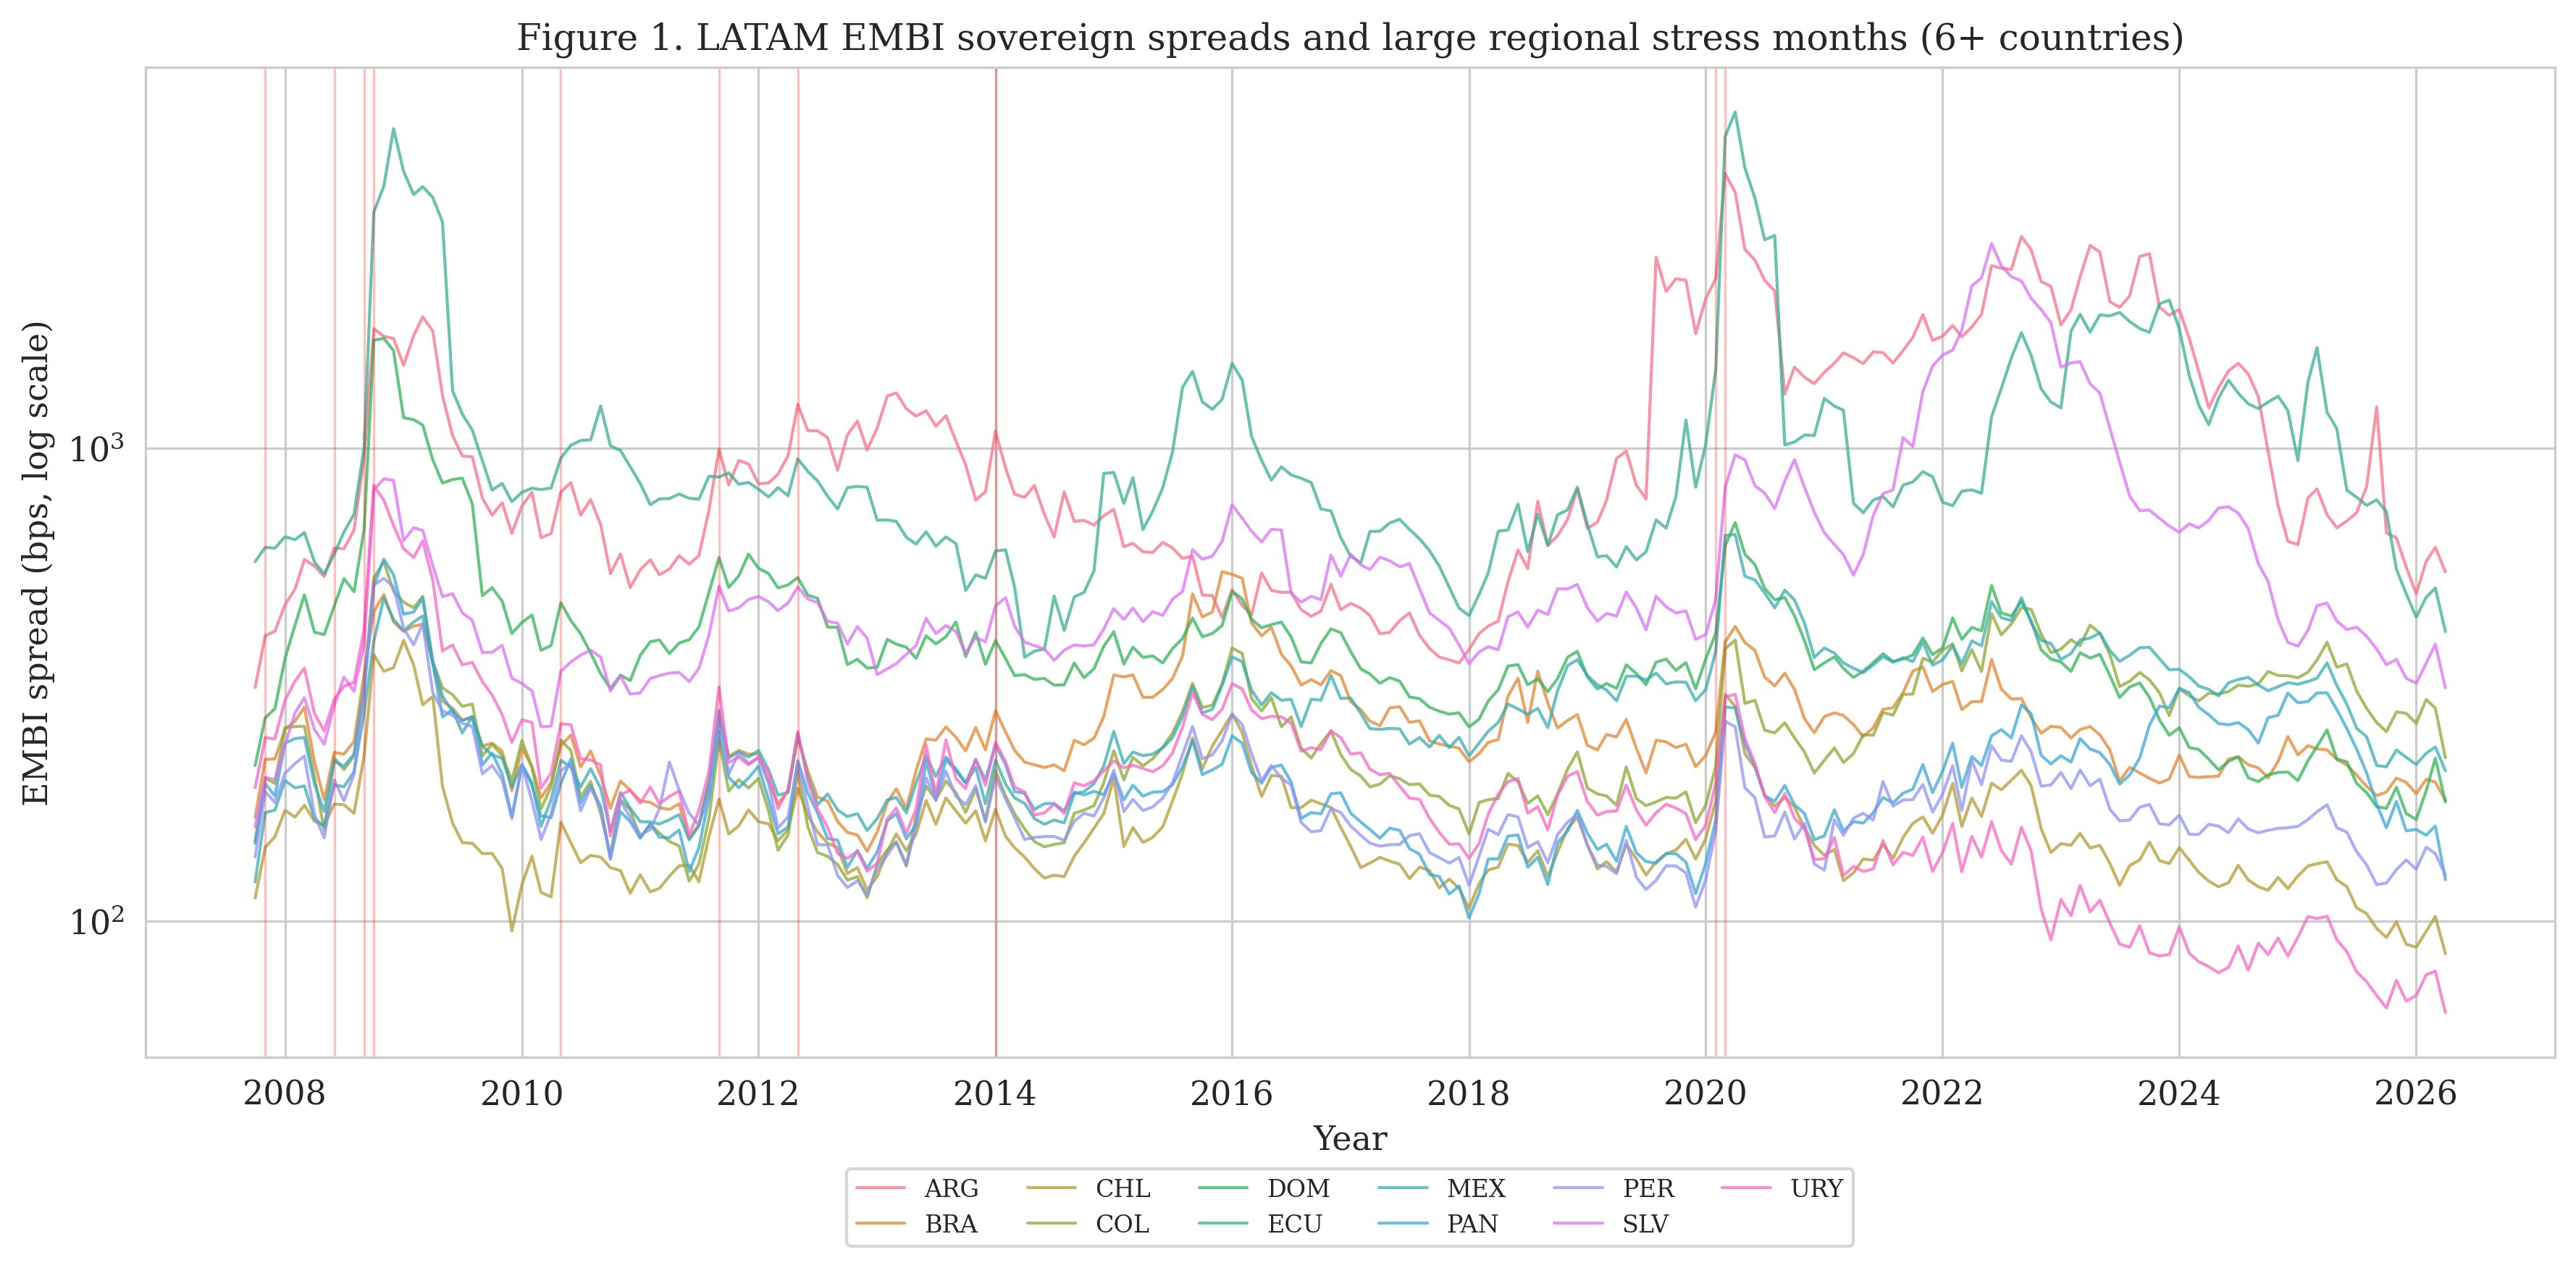
\includegraphics[width=\linewidth]{fig1_latam_spreads.png}
\caption{LATAM EMBI Global Diversified sovereign spreads, 2007:M10--2026:M4
(monthly, basis points, log scale). Vertical red lines mark large regional
stress months ($S_t\geq 6$).}
\label{fig:spreads}
\end{figure}

% =============================================================================
\section{Methodology}
\label{sec:methods}

\subsection{Avalanche identification}
For each country $c$ we compute the standard deviation $\hat{\sigma}_c$ of
the monthly log-change series $\dlogs_{c,t}$ over the full sample. A stress
event is identified when $\dlogs_{c,t} > \sigma\,\hat{\sigma}_c$ with
$\sigma=1.5$ (baseline). Robustness in Section \ref{sec:results} repeats the
analysis for $\sigma\in\{1.25, 1.50, 1.75, 2.00, 2.25, 2.50\}$. The avalanche
size $S_t$ is the cardinality of the set of stressed countries at month $t$.

\subsection{Power-law estimation and tail tests}
For each statistical object $X\in\{S_t,\,|\Delta s_{c,t}|,\,\tau_{c,k}\}$ where
$\tau_{c,k}$ denotes the inter-event time between consecutive stress events
of country $c$, we estimate the maximum-likelihood power-law exponent
$\hat{\alpha}$ and lower cutoff $x_{\min}$ following \citet{Clauset2009}. The
optimal $x_{\min}$ minimizes the Kolmogorov--Smirnov distance between the
empirical and fitted CCDFs. We then conduct \citet{Vuong1989} non-nested tests
against lognormal and exponential alternatives, reporting the normalized
log-likelihood ratio $R$ and one-sided $p$-value. Following the framework of
\citet{StumpfPorter2012}, we treat $|R_{\mathrm{PL/LN}}|<1.5$ as evidence of
the heavy-tail boundary regime in which power-law cannot be discriminated
from lognormal.

\subsection{Filtered networks}
For each rolling window of 24 months ending at month $t$, we compute three
networks. The \emph{correlation network} $G_t^{\rho}$ contains edge $(i,j)$
if and only if $|\hat{\rho}_{ij,t}|>0.4$, with weight $|\hat{\rho}_{ij,t}|$.
The \emph{partial correlation network} $G_t^{\mathrm{part}}$ uses the same
threshold on the partial correlation matrix obtained by inverting the
sample covariance matrix \citep{Mantegna1999}. The
\emph{minimum spanning tree} $G_t^{\mathrm{MST}}$ is the spanning tree of
minimum total distance with $d_{ij}=1-|\hat{\rho}_{ij,t}|$
\citep{Tumminello2005}. The MST has exactly $n-1=10$ edges by construction.

\subsection{Network geometry}
For each network and snapshot we compute (i) the mean Forman--Ricci curvature
$\bar{\kappa}_t^F$ via Equation \eqref{eq:forman}; (ii) the mean
Ollivier--Ricci curvature $\bar{\kappa}_t^O$ via earth-mover linear
programming on neighborhood measures; (iii) the spectral radius $\rho_t$ in
two normalizations and the corresponding $\mathrm{SFI}_t$; (iv) network
density and (v) the Herfindahl--Hirschman index of node strengths. The
Ollivier--Ricci LP has dimensionality $|N(u)|\times|N(v)|$ per edge and is
solved via the simplex method.

\subsection{Placebo synchronization test}
For each bootstrap replication $b=1,\dots,B$ with $B=1{,}000$, we
independently shuffle the stress indicator $\mathbf{1}[\dlogs_{c,t}>\sigma\hat{\sigma}_c]$
across calendar months \emph{within country}. The shuffling preserves
country-level stress frequency by construction but destroys cross-country
synchronization. For each replication we compute four synchronization
statistics: the maximum avalanche size $\Stmax^{(b)}$, the mean positive size
$\bar{S}^{(b)}$, and the shares $P(S\geq 4)^{(b)}$ and $P(S\geq 6)^{(b)}$. The
$p$-value is the placebo-distribution probability of equaling or exceeding
the observed value.

\subsection{Lead-lag predictive analysis}
For each network metric $x_t$ at snapshot $t$, we compute the
contemporaneous Pearson correlation with the maximum avalanche size in the
subsequent three months,
$y_t = \max_{u\in (t,\,t+3]} S_u$, retaining all snapshots with $y_t$
defined.

% =============================================================================
\section{Empirical Results}
\label{sec:results}

\subsection{Heterogeneous country participation (H1, H2)}

Table \ref{tab:country_thresholds} summarizes country-specific stress
thresholds and event counts. The eleven sovereigns participate in stress
events at significantly different rates: Brazil (18 events) is at the top of
the distribution, followed by Mexico (16), Peru (16), Colombia (14) and
Panama (14). The Dominican Republic (7 events) sits at the bottom. A
$\chi^2$ test against uniform participation rejects at $p<0.001$, confirming
H1.

\begin{table}[!htbp]
\centering
\footnotesize
\begin{threeparttable}
\caption{Country-specific stress thresholds and observed event counts, $\sigma=1.5$ specification.}
\label{tab:country_thresholds}
\begin{tabular}{llrrrrrrr}
\toprule
Code & Country & $\sigma_{\Delta\log s}$ & Threshold & $N_c$ & Hit rate & Mean $|\Delta s|$ (bp) & P95 $|\Delta s|$ (bp) & Max $|\Delta s|$ (bp) \\
\midrule
BRA & Brazil & 0.111 & 0.166 & 18 & 0.081 & 22 & 63 & 138 \\
MEX & Mexico & 0.109 & 0.163 & 16 & 0.072 & 22 & 62 & 281 \\
PER & Peru & 0.135 & 0.203 & 16 & 0.072 & 20 & 50 & 203 \\
COL & Colombia & 0.131 & 0.197 & 14 & 0.063 & 24 & 61 & 213 \\
PAN & Panama & 0.129 & 0.193 & 14 & 0.063 & 20 & 54 & 207 \\
SLV & El Salvador & 0.119 & 0.179 & 13 & 0.059 & 53 & 178 & 431 \\
URY & Uruguay & 0.136 & 0.203 & 12 & 0.054 & 22 & 63 & 421 \\
ARG & Argentina & 0.166 & 0.249 & 10 & 0.045 & 132 & 441 & 1,751 \\
CHL & Chile & 0.117 & 0.175 & 10 & 0.045 & 15 & 37 & 142 \\
ECU & Ecuador & 0.195 & 0.293 & 10 & 0.045 & 153 & 448 & 3,087 \\
DOM & Dom. Rep. & 0.119 & 0.178 & 7 & 0.032 & 37 & 91 & 1,018 \\
\bottomrule
\end{tabular}
\begin{tablenotes}\footnotesize
\item A stress event for country $c$ at month $t$ is defined by $\Delta\log s_{c,t} > \sigma\cdot\hat{\sigma}_c$ where $\hat{\sigma}_c$ is the country-specific standard deviation of monthly log changes.
\item Note the inverse pattern: countries with the largest tail jumps (ARG, ECU) display fewer events because their volatility is concentrated in a small number of regime-defining episodes.
\item Mid-credibility, highly-traded sovereigns (BRA, MEX, PER, COL, PAN) accumulate the largest event counts.
\end{tablenotes}
\end{threeparttable}
\end{table}


The substantively interesting finding concerns H2. Argentina and Ecuador,
the two highest-spread economies in the panel (mean levels of 1{,}094 and
1{,}077 basis points respectively), appear in the bottom half of the
ranking with ten stress events each. Chile ranks alongside them with ten
events. The standard sandpile prediction would assign the most events to
the most-stressed economies; the data deliver the opposite.

The reformulated H2 explanation is structural. ARG and ECU exhibit
volatility concentrated in extreme regime-defining episodes---defaults,
runs on the central bank, FX collapses---that saturate the threshold once
and leave the spread in a high absorbed state from which subsequent
volatility produces few additional crossings. Mid-credibility countries
(BRA, MEX, PER, COL, PAN) are more deeply integrated into global emerging-market
debt markets, exhibit more frequent moderate reactions to global news, and
therefore accumulate more threshold crossings. Figures \ref{fig:recurrence}
and \ref{fig:heatmap} display the temporal pattern. Both confirm that
participation is not driven by fiscal stress but by integration with the
global investor base.

\begin{figure}[H]
\centering
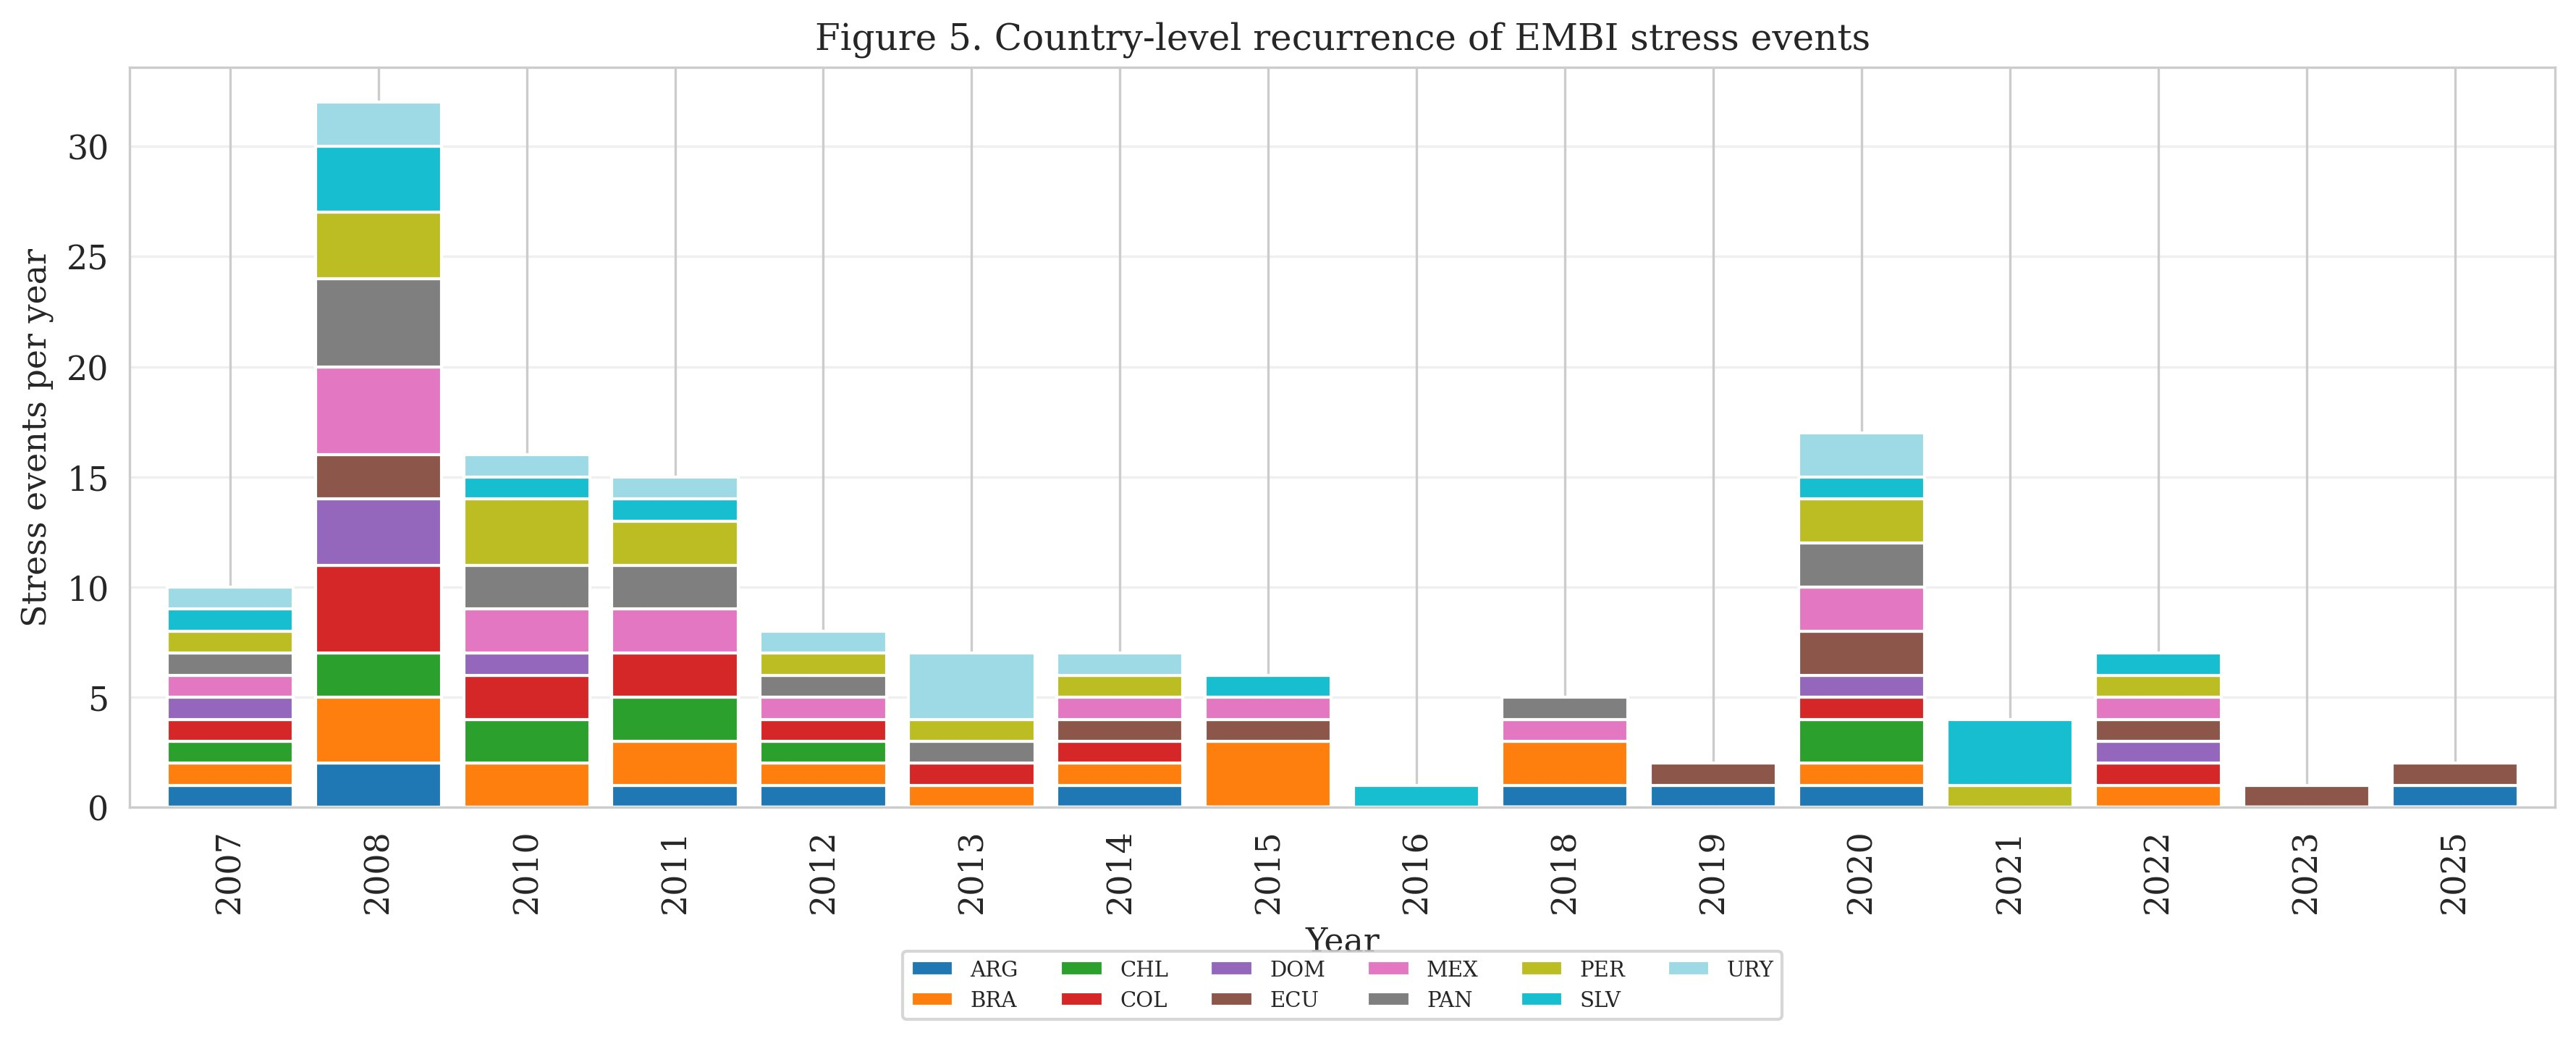
\includegraphics[width=\linewidth]{fig5_country_stress_recurrence.png}
\caption{Country-level recurrence of EMBI stress events by year, stacked
across countries. The 2008 cluster ($n=32$ events), 2010--2011 (Eurozone
crisis) and 2020 (COVID-19) form the three peaks; 2009, 2017 and 2024 are
event-free.}
\label{fig:recurrence}
\end{figure}

\begin{figure}[H]
\centering
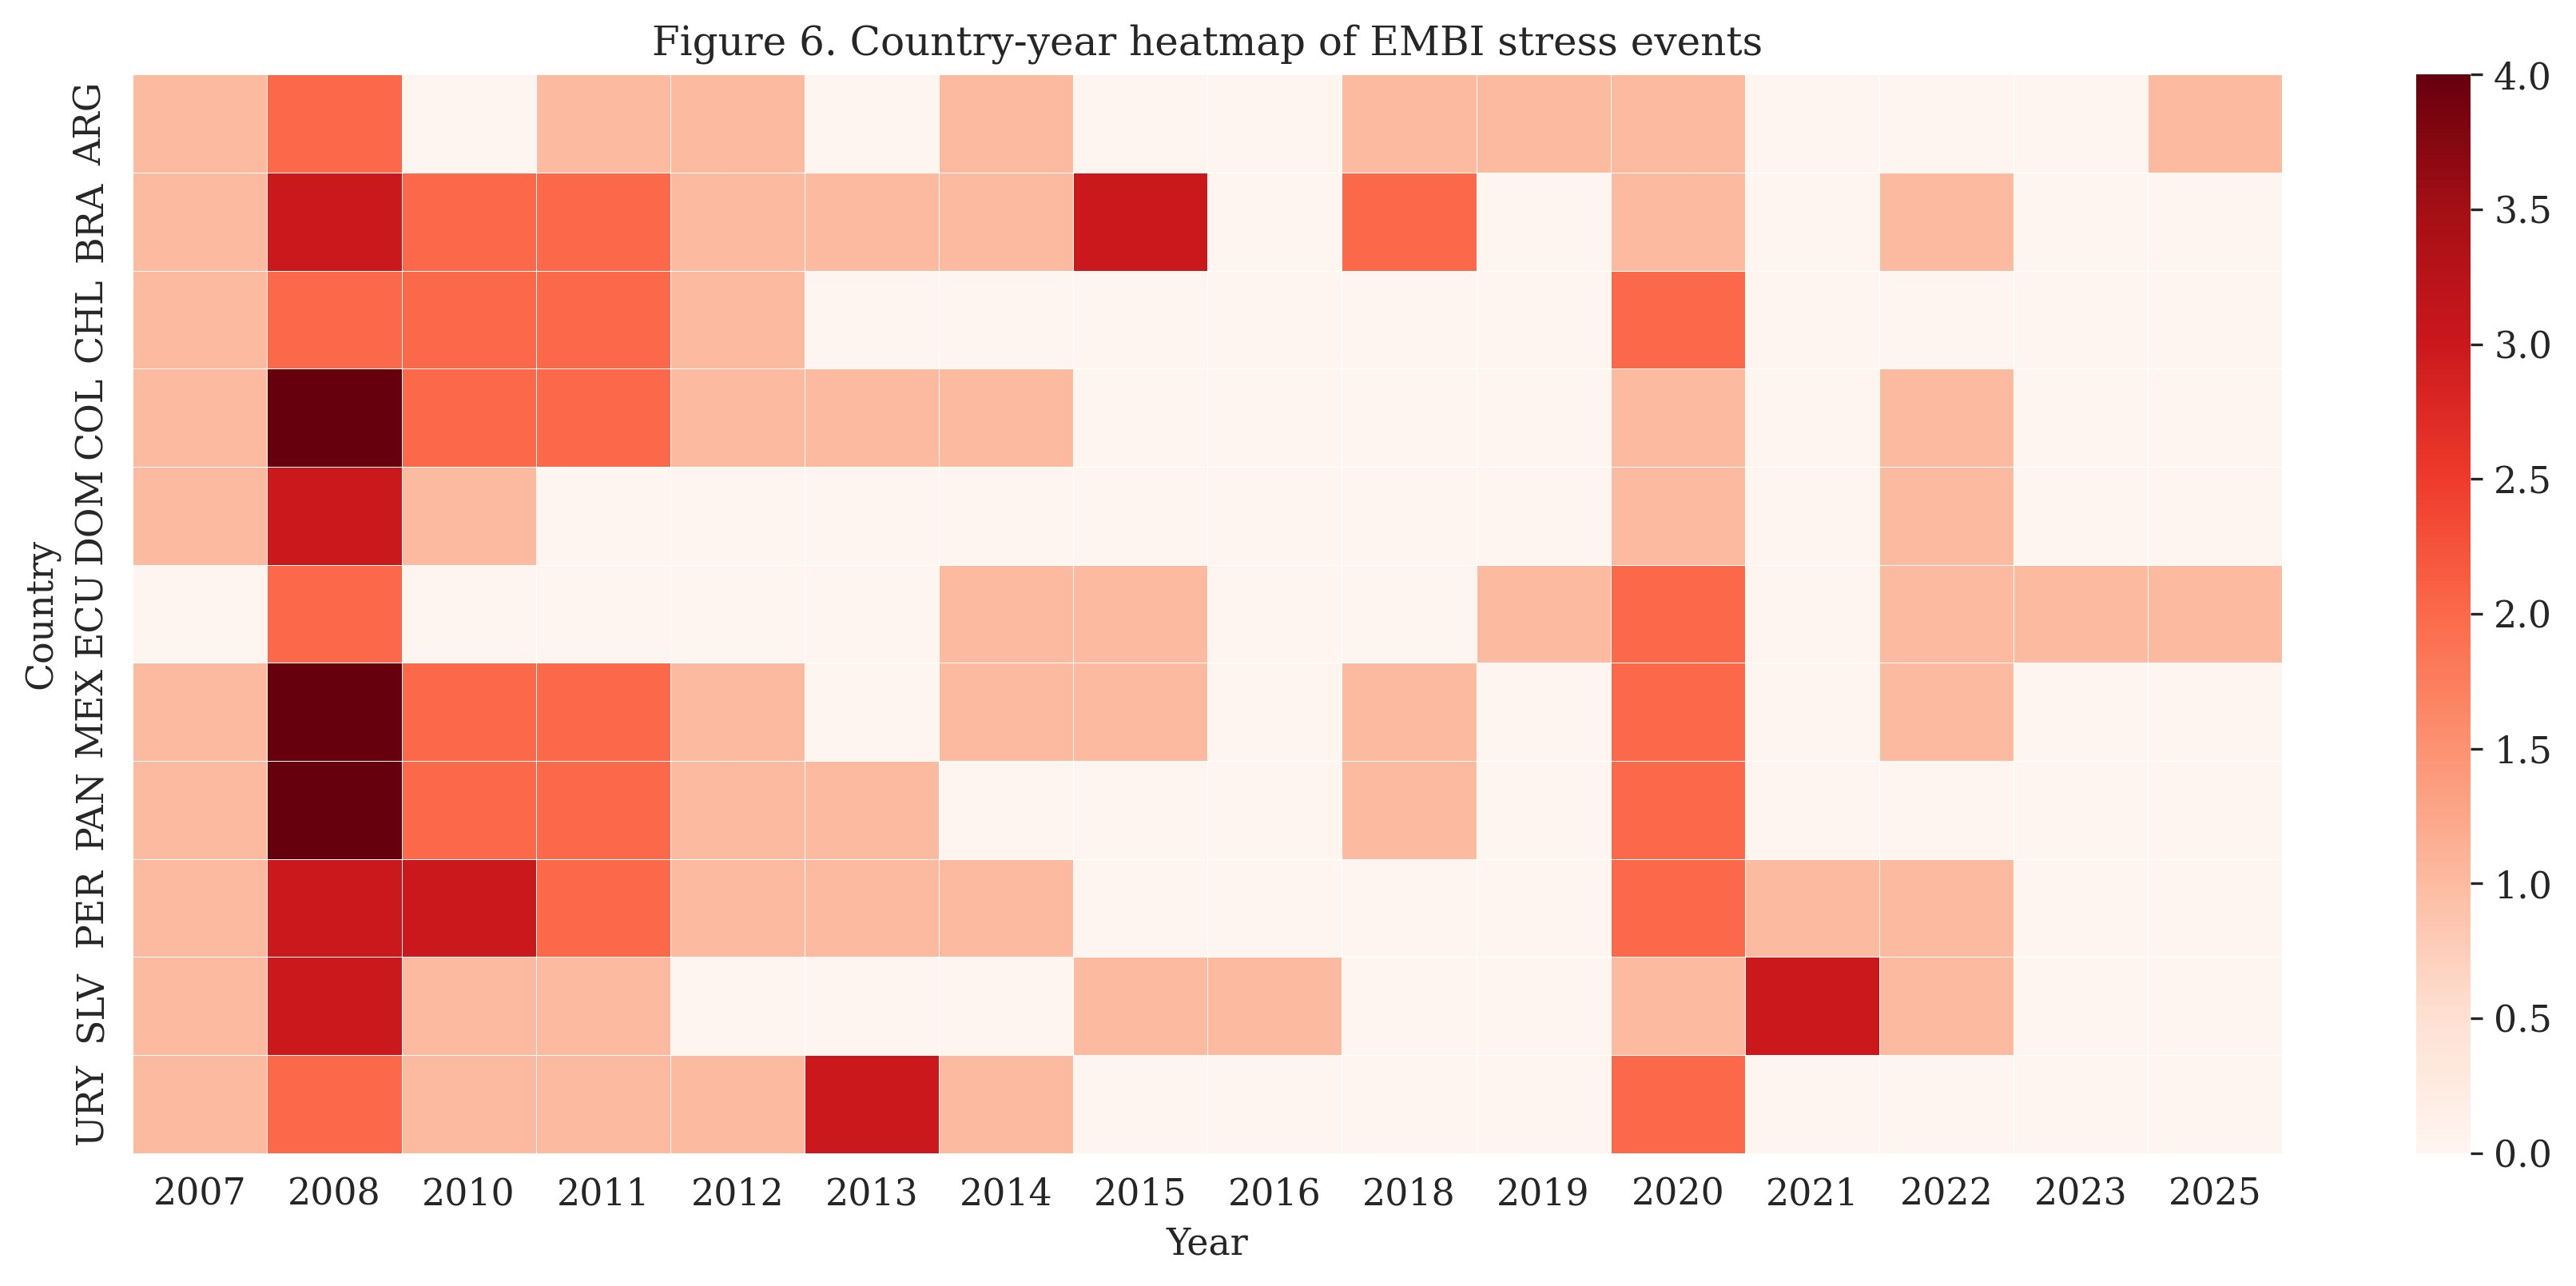
\includegraphics[width=\linewidth]{fig6_stress_heatmap.png}
\caption{Country-year heatmap of EMBI stress events. Cell intensity is the
number of months country $c$ exceeded its $1.5\sigma$ threshold in year $y$.}
\label{fig:heatmap}
\end{figure}

\subsection{Heavy-tail boundary regime (H3)}

Table \ref{tab:tail_diagnostics} reports formal power-law diagnostics for
three statistical objects. The avalanche size distribution yields
$\hat{\alpha}=1.77$ with $x_{\min}=1$. The Vuong test against lognormal
gives $R=-1.61$ with $p_{LN}=0.107$: power-law cannot be rejected. Pooled
absolute spread changes yield $\hat{\alpha}=2.37$ with $x_{\min}=86$ basis
points; $R=-0.76$ with $p_{LN}=0.448$. Inter-event times yield
$\hat{\alpha}=2.38$ with $x_{\min}=12$ months; $R=-0.61$ with $p_{LN}=0.544$.
For all three objects the test statistic is too small to discriminate
between power-law and lognormal alternatives. The data are consistent with
the heavy-tail boundary regime described by \citet{StumpfPorter2012}.

\begin{table}[!htbp]
\centering
\footnotesize
\begin{threeparttable}
\caption{Tail diagnostics for three SOC-relevant statistical objects in LATAM EMBI data, following Clauset, Shalizi, and Newman (2009) and Stumpf and Porter (2012).}
\label{tab:tail_diagnostics}
\begin{tabular}{lrrrrrrrrl}
\toprule
Object & $n$ & $x_{\min}$ & $\hat{\alpha}$ & KS $D$ & $R_{\mathrm{PL/LN}}$ & $p_{\mathrm{LN}}$ & $R_{\mathrm{PL/Exp}}$ & $p_{\mathrm{Exp}}$ & Verdict \\
\midrule
Avalanche size $S_t$ & 40 & 1.000 & 1.771 & 0.095 & -1.612 & 0.107 & -0.502 & 0.616 & Ambiguous \\
$|\Delta s_{c,t}|$ pooled & 2442 & 85.459 & 2.372 & 0.028 & -0.758 & 0.448 & 3.426 & 0.001 & Ambiguous (PL not rejected) \\
Inter-event times (months) & 129 & 11.991 & 2.381 & 0.084 & -0.606 & 0.544 & 1.106 & 0.269 & Ambiguous (PL not rejected) \\
\bottomrule
\end{tabular}
\begin{tablenotes}\footnotesize
\item $\hat{\alpha}$ and $x_{\min}$ are MLE estimates of the power-law tail exponent and the lower cutoff, respectively. KS $D$ is the Kolmogorov--Smirnov distance from the fitted PL above $x_{\min}$.
\item $R_{\mathrm{PL/LN}}$ is the Vuong normalized log-likelihood ratio against a lognormal alternative ($R>0$ favours PL); $|R|<1.5$ indicates the test cannot discriminate.
\item All three objects are consistent with a heavy-tail boundary regime: PL is not rejected against LN at conventional levels, while PL is preferred over an exponential alternative.
\end{tablenotes}
\end{threeparttable}
\end{table}


Figure \ref{fig:avalanche_soc} (Panel A) shows the empirical avalanche-size
CCDF on log-log scale with the fitted power law. Panel B confirms the
country-participation heterogeneity discussed above. Figure
\ref{fig:dspread_diagnostic} reproduces the equivalent analysis for pooled
$|\Delta s|$. The Frobenius normalization of the CCDF and the lognormal
fit superimposed in Panel B are both visually plausible---a graphical
manifestation of the heavy-tail boundary regime that resists statistical
discrimination.

\begin{figure}[H]
\centering
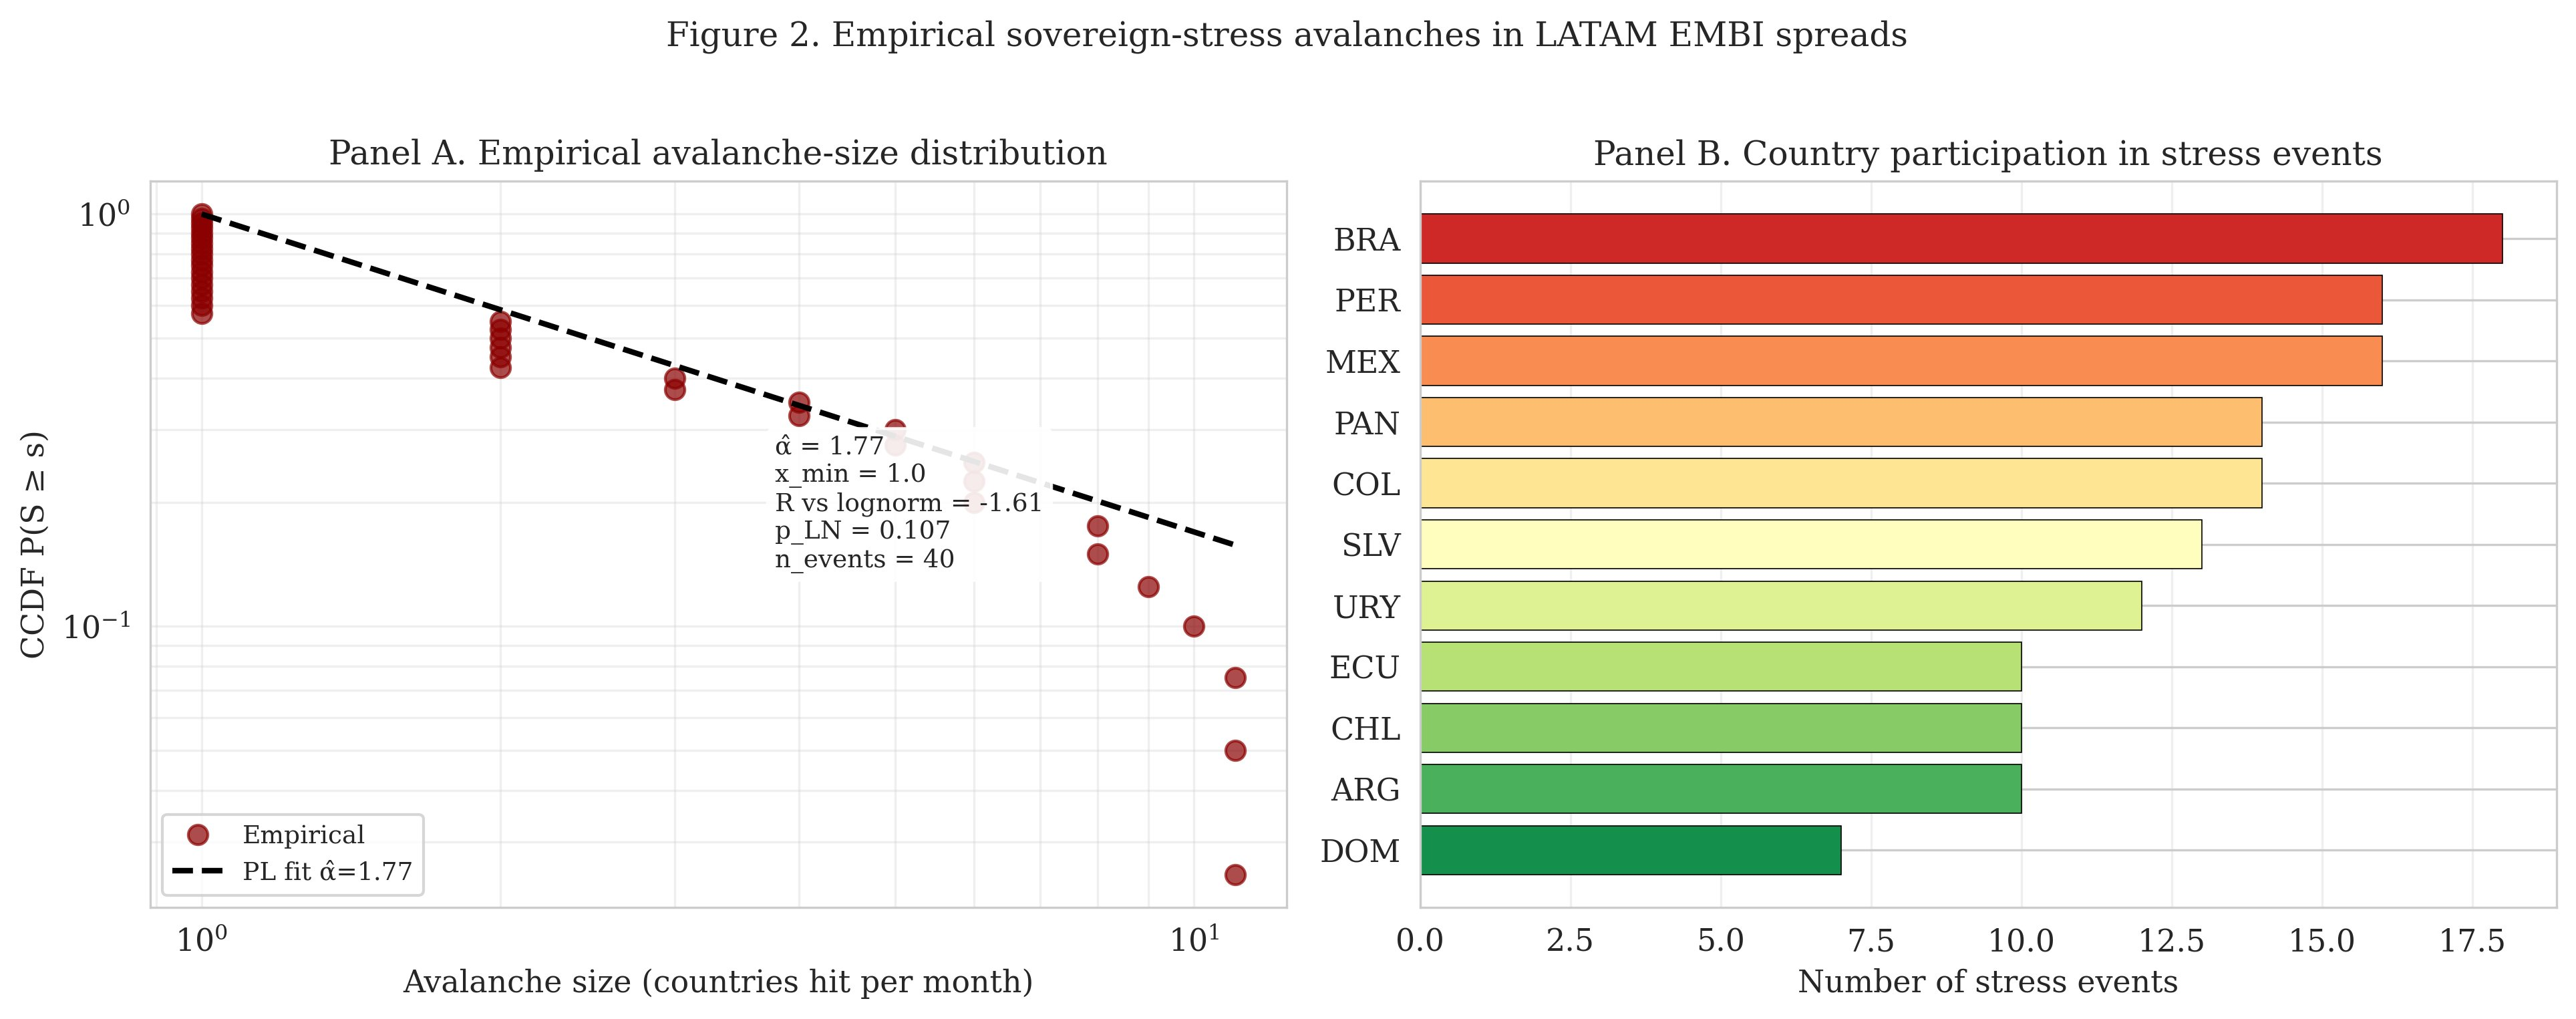
\includegraphics[width=\linewidth]{fig2_avalanche_soc.png}
\caption{Empirical sovereign-stress avalanches in LATAM EMBI spreads. Panel
A: avalanche-size CCDF with maximum-likelihood power-law fit
($\hat{\alpha}=1.77$). Panel B: country participation by stress-event count.}
\label{fig:avalanche_soc}
\end{figure}

\begin{figure}[H]
\centering
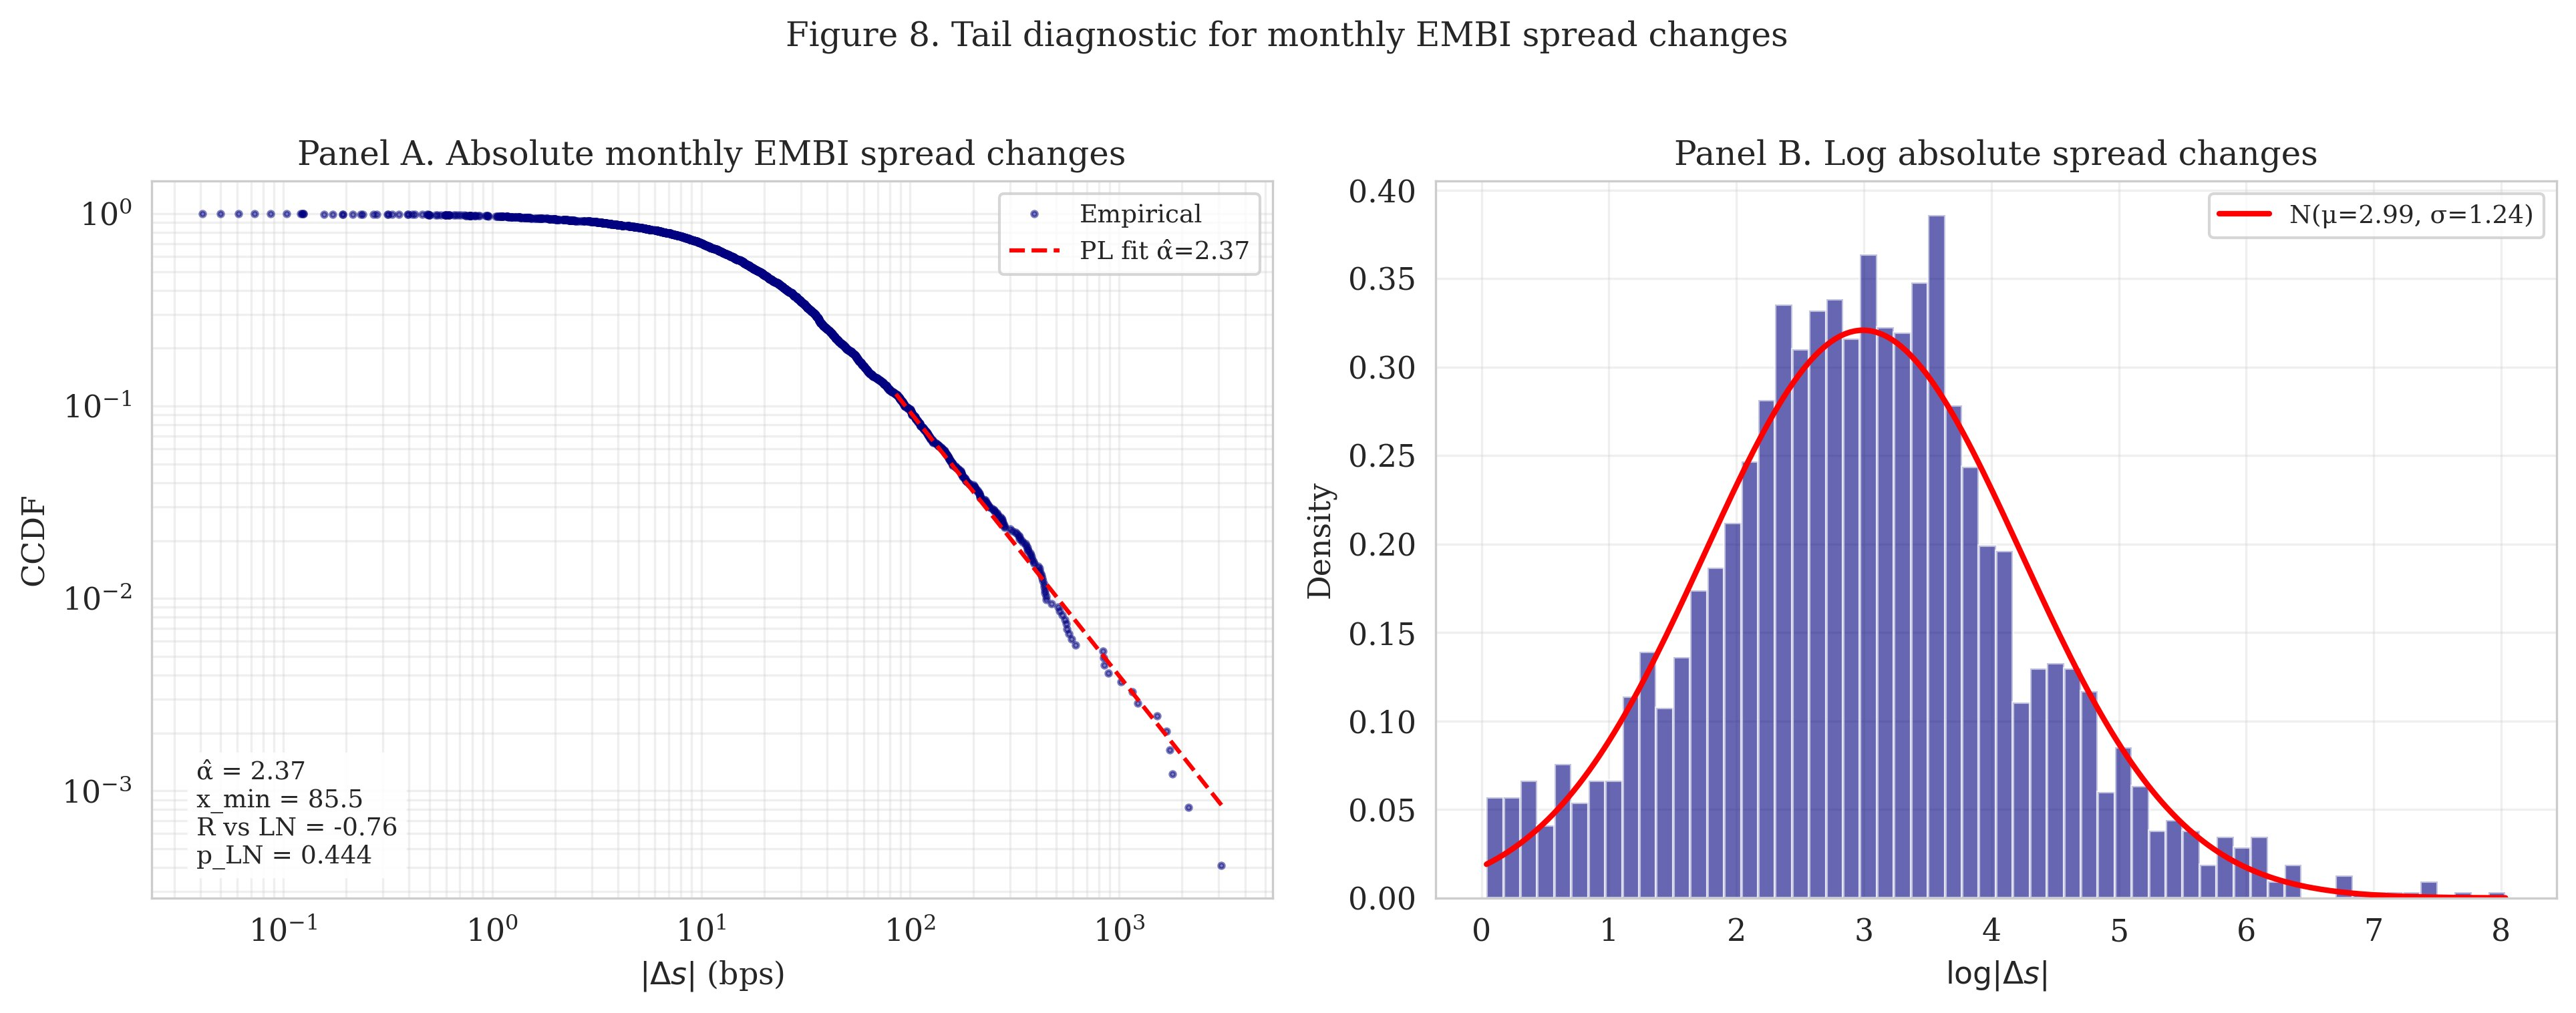
\includegraphics[width=\linewidth]{fig8_dspread_diagnostic.png}
\caption{Tail diagnostic for monthly EMBI spread changes. Panel A: pooled
absolute spread changes with power-law fit ($\hat{\alpha}=2.37$, $x_{\min}=86$
bps). Panel B: log-absolute spread changes histogram with normal
overlay---the heavy-tail boundary regime in graphical form.}
\label{fig:dspread_diagnostic}
\end{figure}

The estimated avalanche tail exponent $\hat{\alpha}=1.77$ falls inside the
canonical SOC range $[1, 3]$ \citep{Bak1996, NewmanPL2005}, consistent with
the prediction of \citet{Bak1993} for sandpile-like economic systems.

\subsection{Synchronization is non-trivial (H4)}

Table \ref{tab:placebo} reports the reshuffle-placebo test. Under independent
country-level stress with preserved frequencies, the placebo distribution of
the maximum avalanche size has mean 3.47 and 95th percentile 4. The observed
$\Stmax=11$ is unattainable in the placebo distribution. All four
synchronization statistics yield $p<0.001$, decisively rejecting the
independence null. Cross-country LATAM stress synchronization is genuinely
multi-country, not a coincidence of independent national reactions to common
news.

\begin{table}[!htbp]
\centering
\footnotesize
\begin{threeparttable}
\caption{Placebo test of cross-country stress synchronization. Country-level stress indicators are independently reshuffled across calendar months, breaking common-shock structure while preserving country-level event frequencies.}
\label{tab:placebo}
\begin{tabular}{lrrrr}
\toprule
Statistic & Observed & Placebo mean & Placebo P95 & $p$-value \\
\midrule
Max avalanche size $S_{\max}$ & 11 & 3.47 & 4.00 & 0.000 \\
Mean avalanche size $\bar{S}$ & 3.50 & 1.32 & 1.40 & 0.000 \\
Share $P(S\geq 4)$ & 0.350 & 0.005 & 0.019 & 0.000 \\
Share $P(S\geq 6)$ & 0.250 & 0.000 & 0.000 & 0.000 \\
\bottomrule
\end{tabular}
\begin{tablenotes}\footnotesize
\item Bootstrap replications: $B=1000$, seed $=2026$.
\item Under the null of independent country-level stress, the maximum simultaneously-hit panel is at most $\bar{S}_{\max}^{\mathrm{pl}}\approx 3.5$. The observed value $S_{\max}=11$ is unattainable in the placebo distribution.
\item All four synchronization statistics reject the independence null at $p<0.001$, confirming that simultaneous LATAM stress is a non-trivial multi-country phenomenon.
\end{tablenotes}
\end{threeparttable}
\end{table}


Table \ref{tab:top_avalanches} lists the twelve largest avalanches with
historical context. The three avalanches of size $S=11$ all coincide with
documented global systemic events: the Lehman collapse (September 2008), the
post-Lehman EM rout (October 2008) and the COVID-19 global rout (March 2020).
Every avalanche of size $S\geq 9$ corresponds to an identifiable
international stress episode. The empirical avalanche structure is therefore
not a statistical artefact: it tracks the historical timeline of
international financial volatility.

\begin{table}[!htbp]
\centering
\footnotesize
\begin{threeparttable}
\caption{Top 12 largest empirical avalanches in LATAM EMBI spreads, with historical context.}
\label{tab:top_avalanches}
\begin{tabular}{rlrp{0.30\linewidth}p{0.32\linewidth}}
\toprule
Rank & Month & $S_t$ & Countries hit & Historical context \\
\midrule
1 & 2020-03 & 11 & ARG, BRA, CHL, COL, DOM, ECU, MEX, PAN, PER, SLV, URY & COVID-19 global rout, Ecuador default \\
2 & 2008-09 & 11 & ARG, BRA, CHL, COL, DOM, ECU, MEX, PAN, PER, SLV, URY & Lehman collapse (global GFC peak) \\
3 & 2008-10 & 11 & ARG, BRA, CHL, COL, DOM, ECU, MEX, PAN, PER, SLV, URY & Post-Lehman EM rout \\
4 & 2007-11 & 10 & ARG, BRA, CHL, COL, DOM, MEX, PAN, PER, SLV, URY & Pre-crisis volatility wave (Bear Stearns hedge funds collapse) \\
5 & 2011-09 & 9 & ARG, BRA, CHL, COL, MEX, PAN, PER, SLV, URY & Eurozone crisis intensifies \\
6 & 2010-05 & 8 & BRA, CHL, COL, DOM, MEX, PER, SLV, URY & Eurozone crisis (first Greek bailout) \\
7 & 2012-05 & 8 & ARG, BRA, CHL, COL, MEX, PAN, PER, URY & Greek collapse round II \\
8 & 2008-06 & 6 & BRA, COL, MEX, PAN, PER, SLV & Subprime spillover to EM \\
9 & 2020-02 & 6 & CHL, ECU, MEX, PAN, PER, URY & COVID-19 onset, Ecuador default brewing \\
10 & 2014-01 & 6 & ARG, BRA, COL, MEX, PER, URY & EM Fragile Five sell-off \\
11 & 2011-08 & 5 & BRA, CHL, COL, MEX, PAN & U.S. debt-ceiling / S\&P downgrade \\
12 & 2022-06 & 5 & BRA, COL, DOM, ECU, MEX & Fed front-loading; LATAM commodity stress \\
\bottomrule
\end{tabular}
\begin{tablenotes}\footnotesize
\item Each row is a calendar month ranked by $S_t$ = number of countries simultaneously exceeding their $1.5\sigma$ threshold.
\item Every avalanche of size $S\geq 9$ coincides with a documented global systemic event.
\item All $S=11$ months are universal-stress events (every LATAM sovereign in the panel hit simultaneously).
\end{tablenotes}
\end{threeparttable}
\end{table}


\subsection{Network geometry and regime change (H5)}

Figure \ref{fig:networks} displays the three filtered networks at four
representative dates. The October 2009 (post-GFC) snapshot reveals near-full
density across all three filters. The April 2018 snapshot, capturing the
Argentine pre-IMF crisis, shows ARG isolated as a disconnected node in the
correlation network and weakly tied in the partial correlation
network---a graphical illustration of the country's idiosyncratic decoupling
prior to the 2019 PASO shock. The April 2021 snapshot, capturing the
post-COVID recovery, shows partial restoration of connectivity.

\begin{figure}[H]
\centering
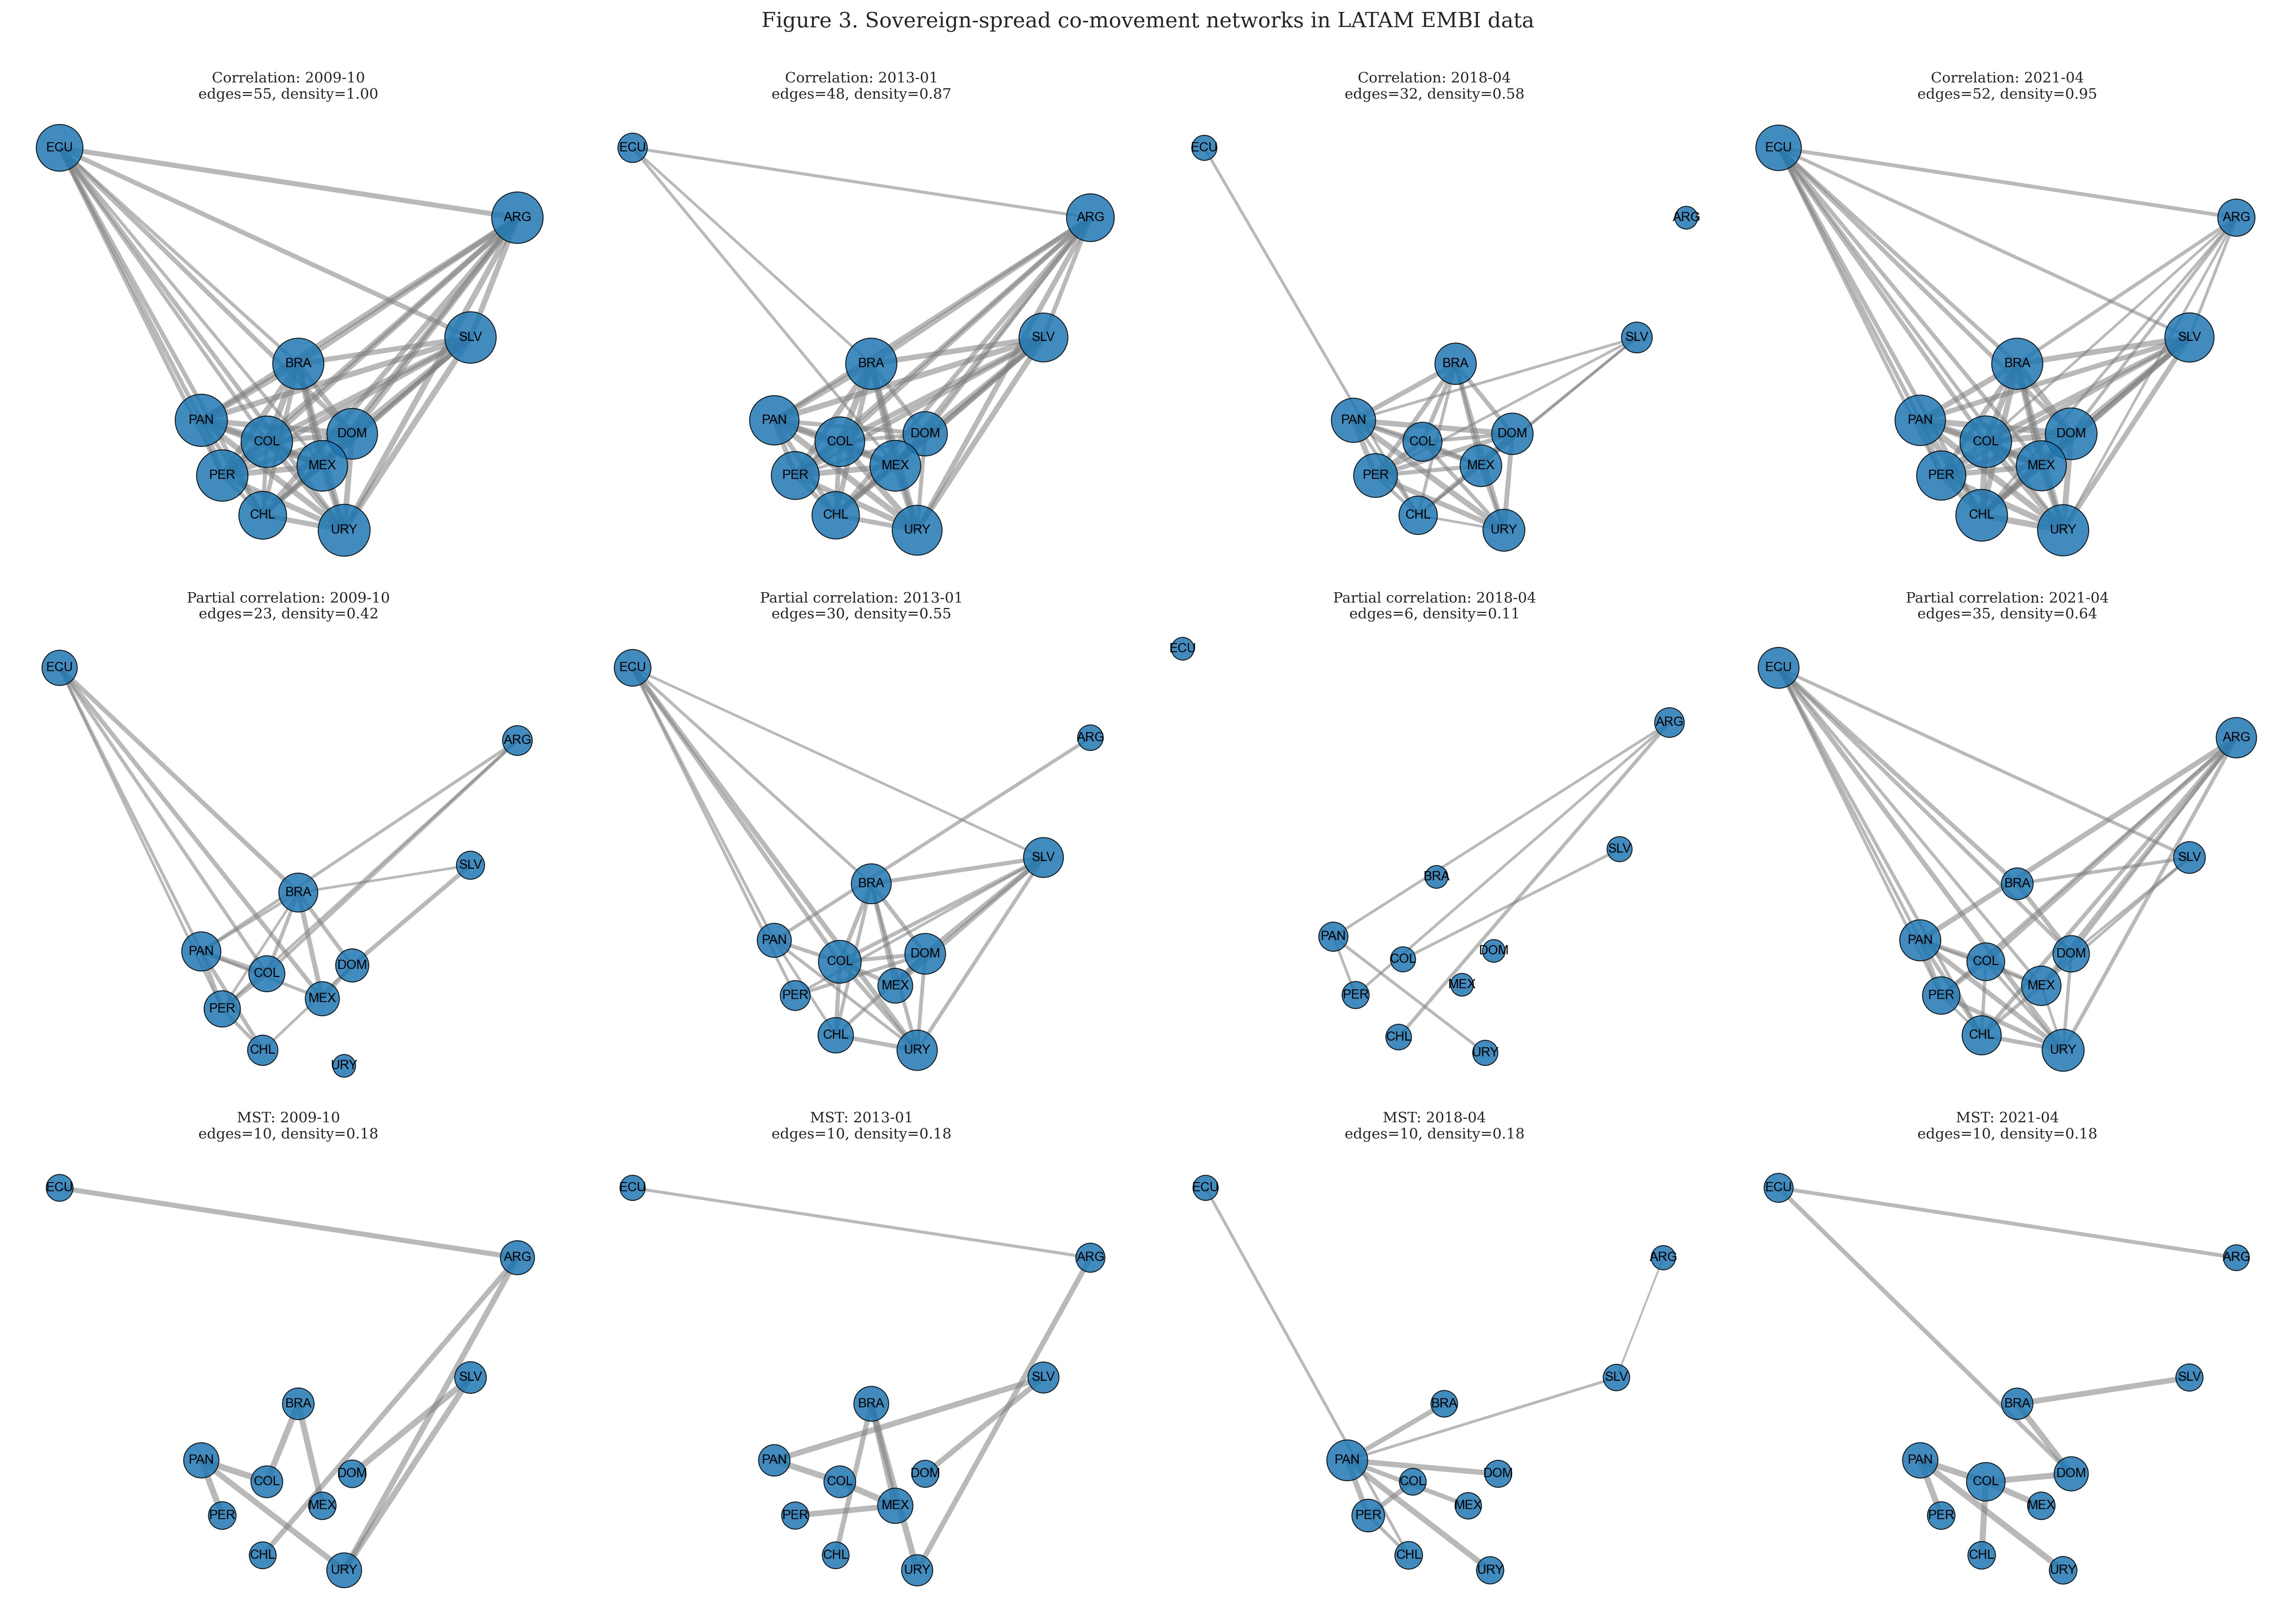
\includegraphics[width=\linewidth]{fig3_network_snapshots.png}
\caption{Sovereign-spread co-movement networks in LATAM EMBI data, four
representative dates. Top row: correlation network. Middle row: partial
correlation network. Bottom row: minimum spanning tree.}
\label{fig:networks}
\end{figure}

Figure \ref{fig:geometry} traces the dynamics of network geometry through
2009--2026. Panel A shows the mean Ollivier--Ricci curvature, Panel C the
spectral radius, Panel E the Spectral Fragility Index and Panel F the
density. The partial-correlation network exhibits the most informative
dynamics, with clear regime shifts visible around 2008--2010 and
2020--2022.

\begin{figure}[H]
\centering
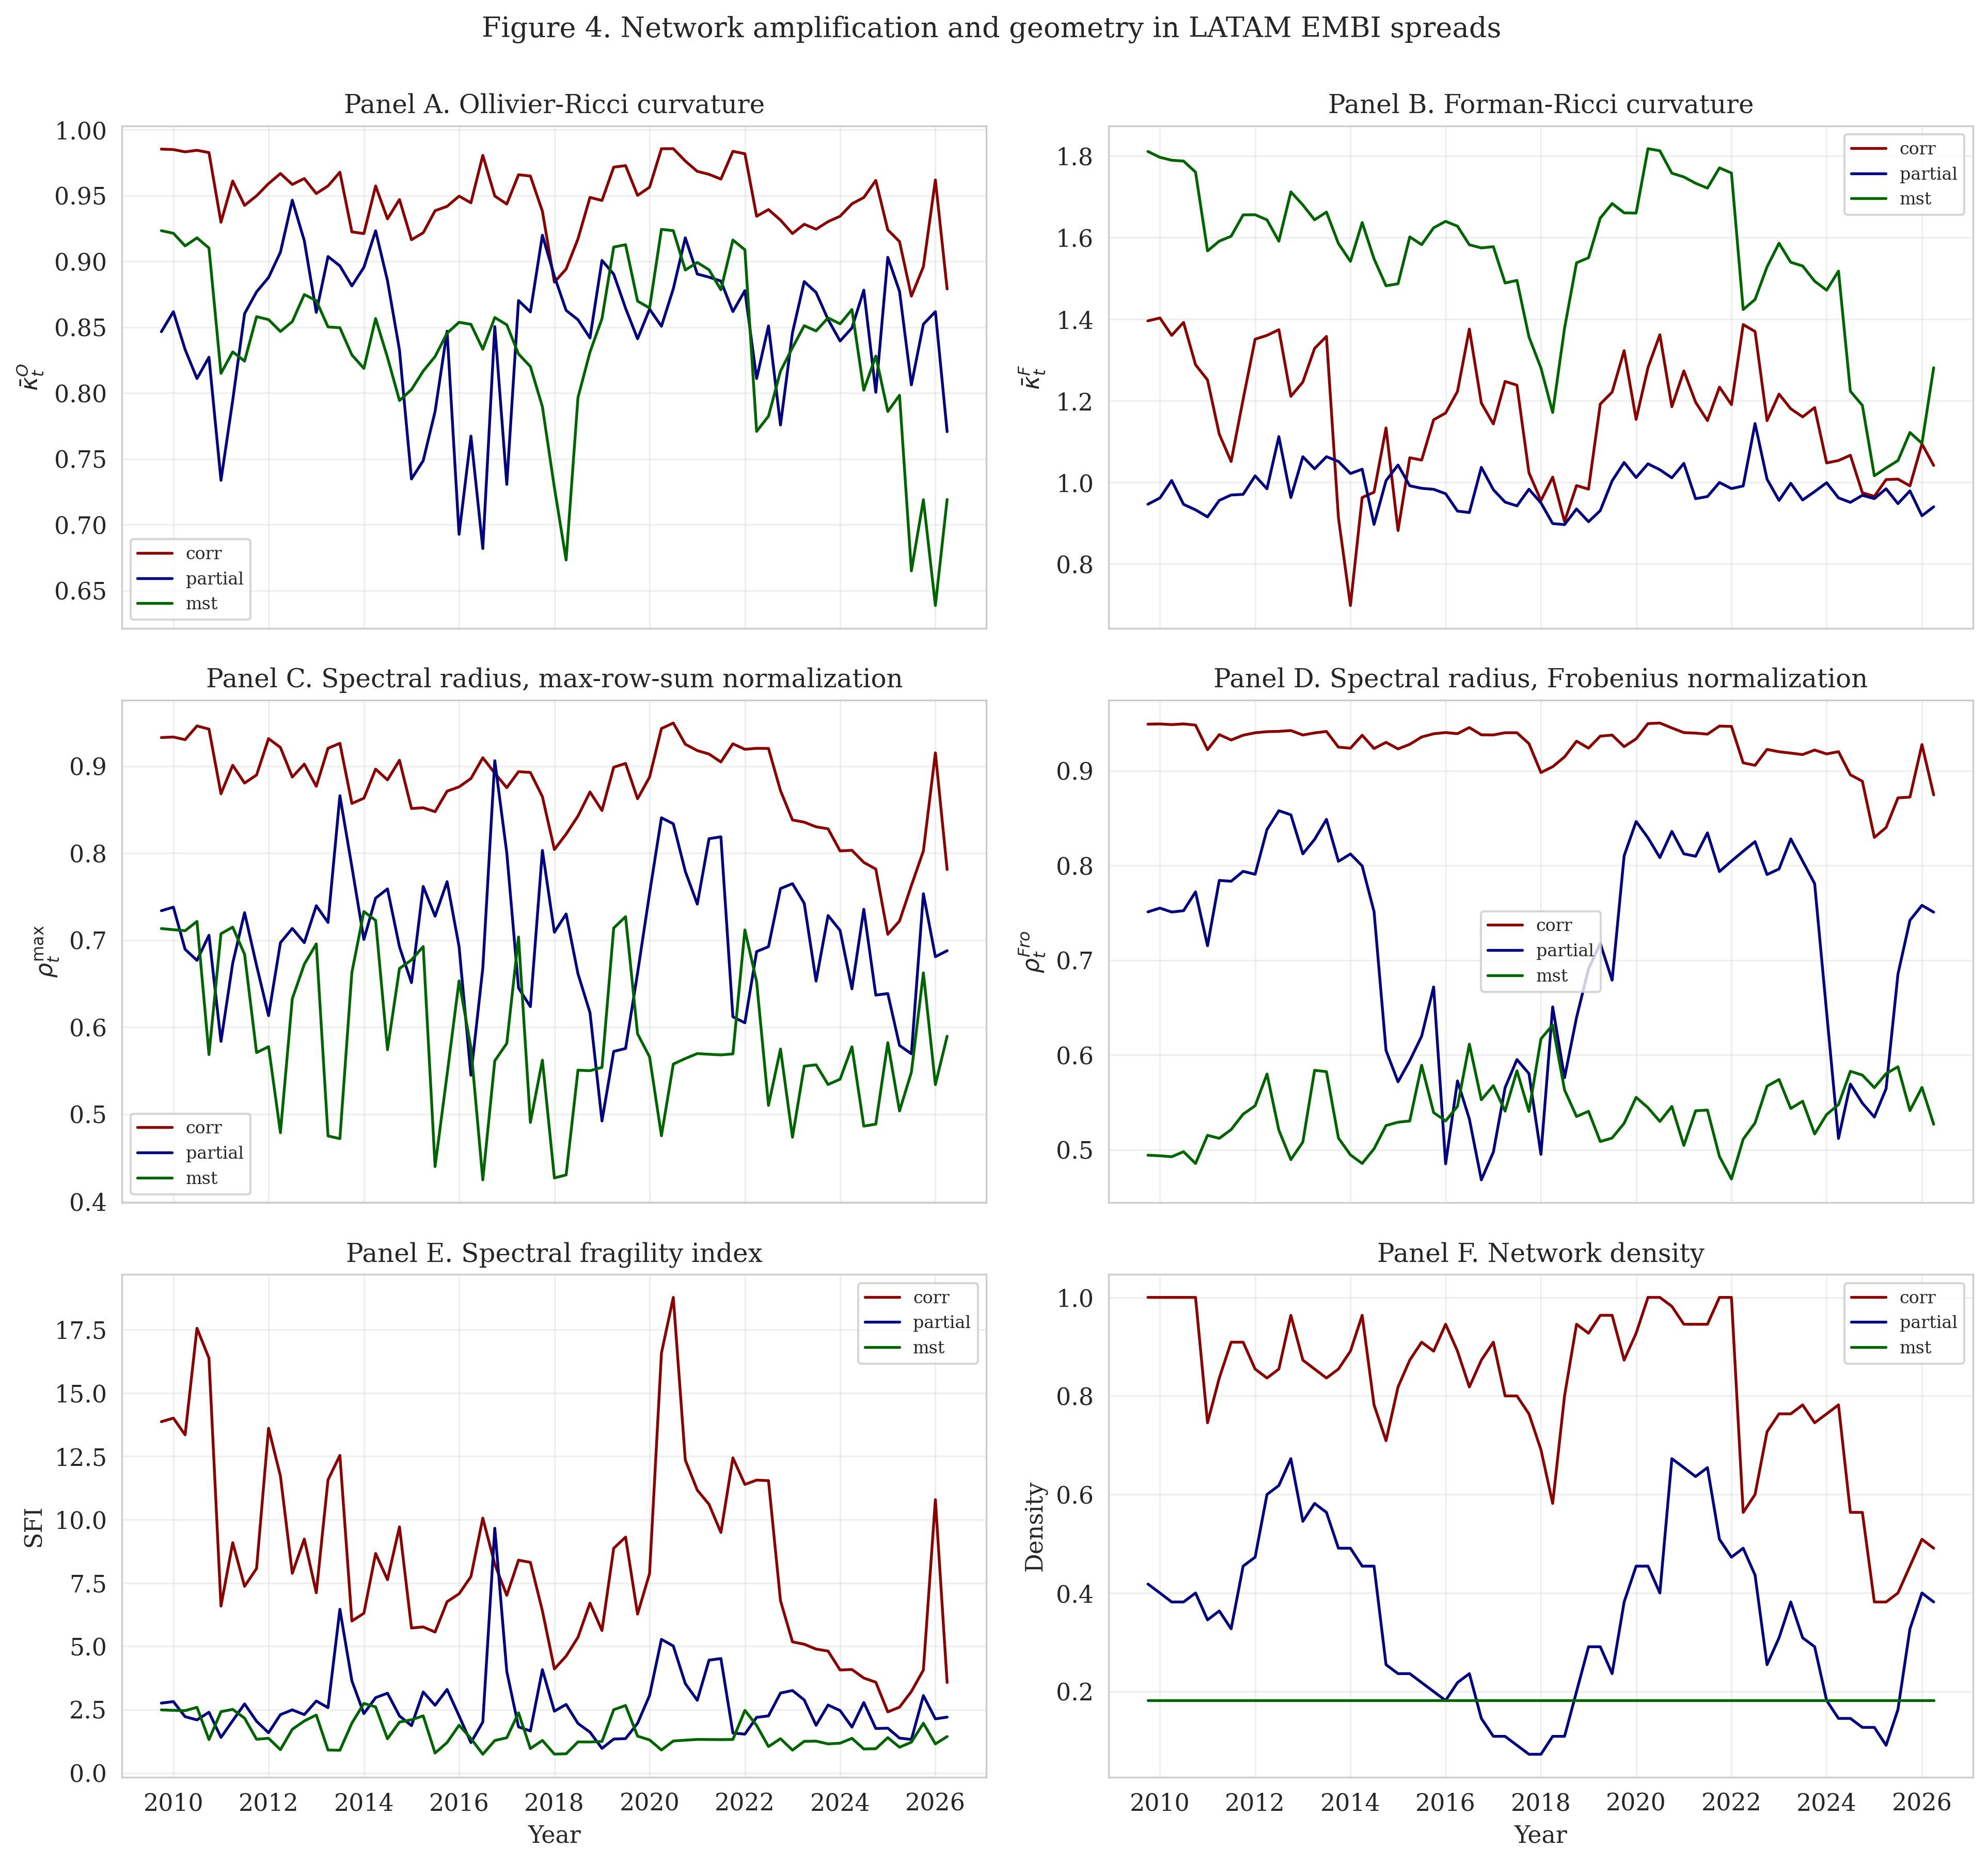
\includegraphics[width=\linewidth]{fig4_geometry_dynamics.png}
\caption{Network amplification and geometry in LATAM EMBI spreads, 2009--2026.}
\label{fig:geometry}
\end{figure}

Table \ref{tab:network_regime} contrasts metric values during 24-month
windows that contain at least one large stress event ($S\geq 6$) against
windows that do not. The partial-correlation network is the only one to yield
consistent and significant differences. Frobenius spectral radius rises from
0.71 in non-large to 0.81 in large windows ($t=4.35$, $p=0.001$); Frobenius
SFI rises from 2.95 to 4.33 ($t=2.75$, $p=0.04$); density rises from 0.33 to
0.45 ($t=2.28$, $p=0.06$); HHI of node strengths falls (more even
participation) from 0.127 to 0.117 ($t=-2.20$, $p=0.05$). The
correlation network shows weaker effects, primarily on density. The MST
network shows no significant regime difference, reflecting its constant
edge count and limited information content.

\begin{table}[!htbp]
\centering
\footnotesize
\begin{threeparttable}
\caption{Network geometry around large stress months. Welch's two-sample $t$-test contrasts metric values in months in the 24-month rolling window centred on a large avalanche ($S\geq 6$) versus all other windows.}
\label{tab:network_regime}
\begin{tabular}{llrrrrrrr}
\toprule
Filter & Metric & Non-large mean & Large mean & $\Delta$ & $t$ & $p$ & $n_L$ & $n_N$ \\
\midrule
corr & $\rho^{\max}$ & 0.847 & 0.911 & 0.065 & 6.259 & 0.000 & 33 & 34 \\
corr & $\rho^{\mathrm{Fro}}$ & 0.913 & 0.941 & 0.027 & 4.607 & 0.000 & 33 & 34 \\
corr & SFI$^{\max}$ & 6.229 & 11.743 & 5.515 & 6.304 & 0.000 & 33 & 34 \\
corr & SFI$^{\mathrm{Fro}}$ & 11.858 & 16.296 & 4.438 & 5.636 & 0.000 & 33 & 34 \\
corr & $\bar{\kappa}^O$ & 0.935 & 0.963 & 0.028 & 4.132 & 0.000 & 33 & 34 \\
corr & $\bar{\kappa}^F$ & 1.138 & 1.254 & 0.116 & 2.547 & 0.014 & 33 & 34 \\
corr & Density & 0.739 & 0.915 & 0.177 & 5.419 & 0.000 & 33 & 34 \\
corr & HHI strength & 0.106 & 0.096 & -0.010 & -4.645 & 0.000 & 33 & 34 \\
partial & $\rho^{\max}$ & 0.871 & 0.855 & -0.015 & -0.786 & 0.435 & 33 & 34 \\
partial & $\rho^{\mathrm{Fro}}$ & 0.914 & 0.896 & -0.018 & -1.480 & 0.144 & 33 & 34 \\
partial & SFI$^{\max}$ & 10.079 & 10.173 & 0.093 & 0.044 & 0.965 & 33 & 34 \\
partial & SFI$^{\mathrm{Fro}}$ & 12.696 & 11.159 & -1.537 & -1.244 & 0.219 & 33 & 34 \\
partial & $\bar{\kappa}^O$ & 0.923 & 0.909 & -0.014 & -0.878 & 0.383 & 33 & 34 \\
partial & $\bar{\kappa}^F$ & 1.262 & 1.230 & -0.032 & -0.533 & 0.596 & 33 & 34 \\
partial & Density & 0.693 & 0.715 & 0.023 & 0.454 & 0.651 & 33 & 34 \\
partial & HHI strength & 0.109 & 0.106 & -0.004 & -1.262 & 0.211 & 33 & 34 \\
mst & $\rho^{\max}$ & 0.562 & 0.614 & 0.052 & 2.832 & 0.006 & 33 & 34 \\
mst & $\rho^{\mathrm{Fro}}$ & 0.558 & 0.516 & -0.042 & -6.453 & 0.000 & 33 & 34 \\
mst & SFI$^{\max}$ & 1.336 & 1.721 & 0.385 & 2.988 & 0.004 & 33 & 34 \\
mst & SFI$^{\mathrm{Fro}}$ & 1.270 & 1.074 & -0.195 & -6.235 & 0.000 & 33 & 34 \\
mst & $\bar{\kappa}^O$ & 0.812 & 0.874 & 0.061 & 4.510 & 0.000 & 33 & 34 \\
mst & $\bar{\kappa}^F$ & 1.445 & 1.689 & 0.245 & 6.208 & 0.000 & 33 & 34 \\
mst & HHI strength & 0.135 & 0.119 & -0.016 & -5.930 & 0.000 & 33 & 34 \\
\bottomrule
\end{tabular}
\begin{tablenotes}\footnotesize
\item Filters refer to the network construction: $|\rho|>0.4$ (corr), partial correlation $>0.4$ (partial), or planar minimum-spanning tree (mst).
\item Network density and edge counts in MST are constant by construction (10 edges among 11 nodes) and are omitted.
\item The partial-correlation network exhibits the strongest large-vs-non-large discrimination, with significant increases in Frobenius spectral radius and Frobenius SFI during large-stress windows.
\end{tablenotes}
\end{threeparttable}
\end{table}


Table \ref{tab:network_predictive} reports lead-lag Pearson correlations
between contemporaneous network metrics and the maximum avalanche size in
the subsequent three months. The partial-correlation Frobenius spectral
radius is the single most predictive metric, with $r=+0.28$ at $p=0.024$.
The partial-correlation Frobenius SFI follows closely with $r=+0.28$ at
$p=0.025$. Density and edge count of the partial-correlation network also
yield significant lead-lag association at the 10\% level. The correlation
network and MST do not show statistically robust predictive structure. This
finding is consistent with the partial-correlation methodology of
\citet{Mantegna1999} and the network-connectedness framework of
\citet{Diebold2014}: information about idiosyncratic propagation channels is
captured in partial correlations after global common-factor variation has
been removed.

\subsection{Threshold robustness (H6)}

Figure \ref{fig:robustness} and Table \ref{tab:threshold_robustness}
document the sensitivity of all quantitative findings to the threshold
parameter $\sigma$. The estimated tail exponent of avalanche size remains
in the range $[1.70, 1.83]$ for $\sigma\leq 2.0$ and rises only modestly to
2.53 at $\sigma=2.25$ where the tail truncation reduces the effective sample.
The maximum avalanche size remains $\Stmax=11$ at every threshold tested,
confirming that universal-stress events (Lehman 2008, COVID-19 2020) are
not artefacts of threshold choice. The Vuong test continues to fail to
reject power-law against lognormal at all thresholds.

\begin{figure}[H]
\centering
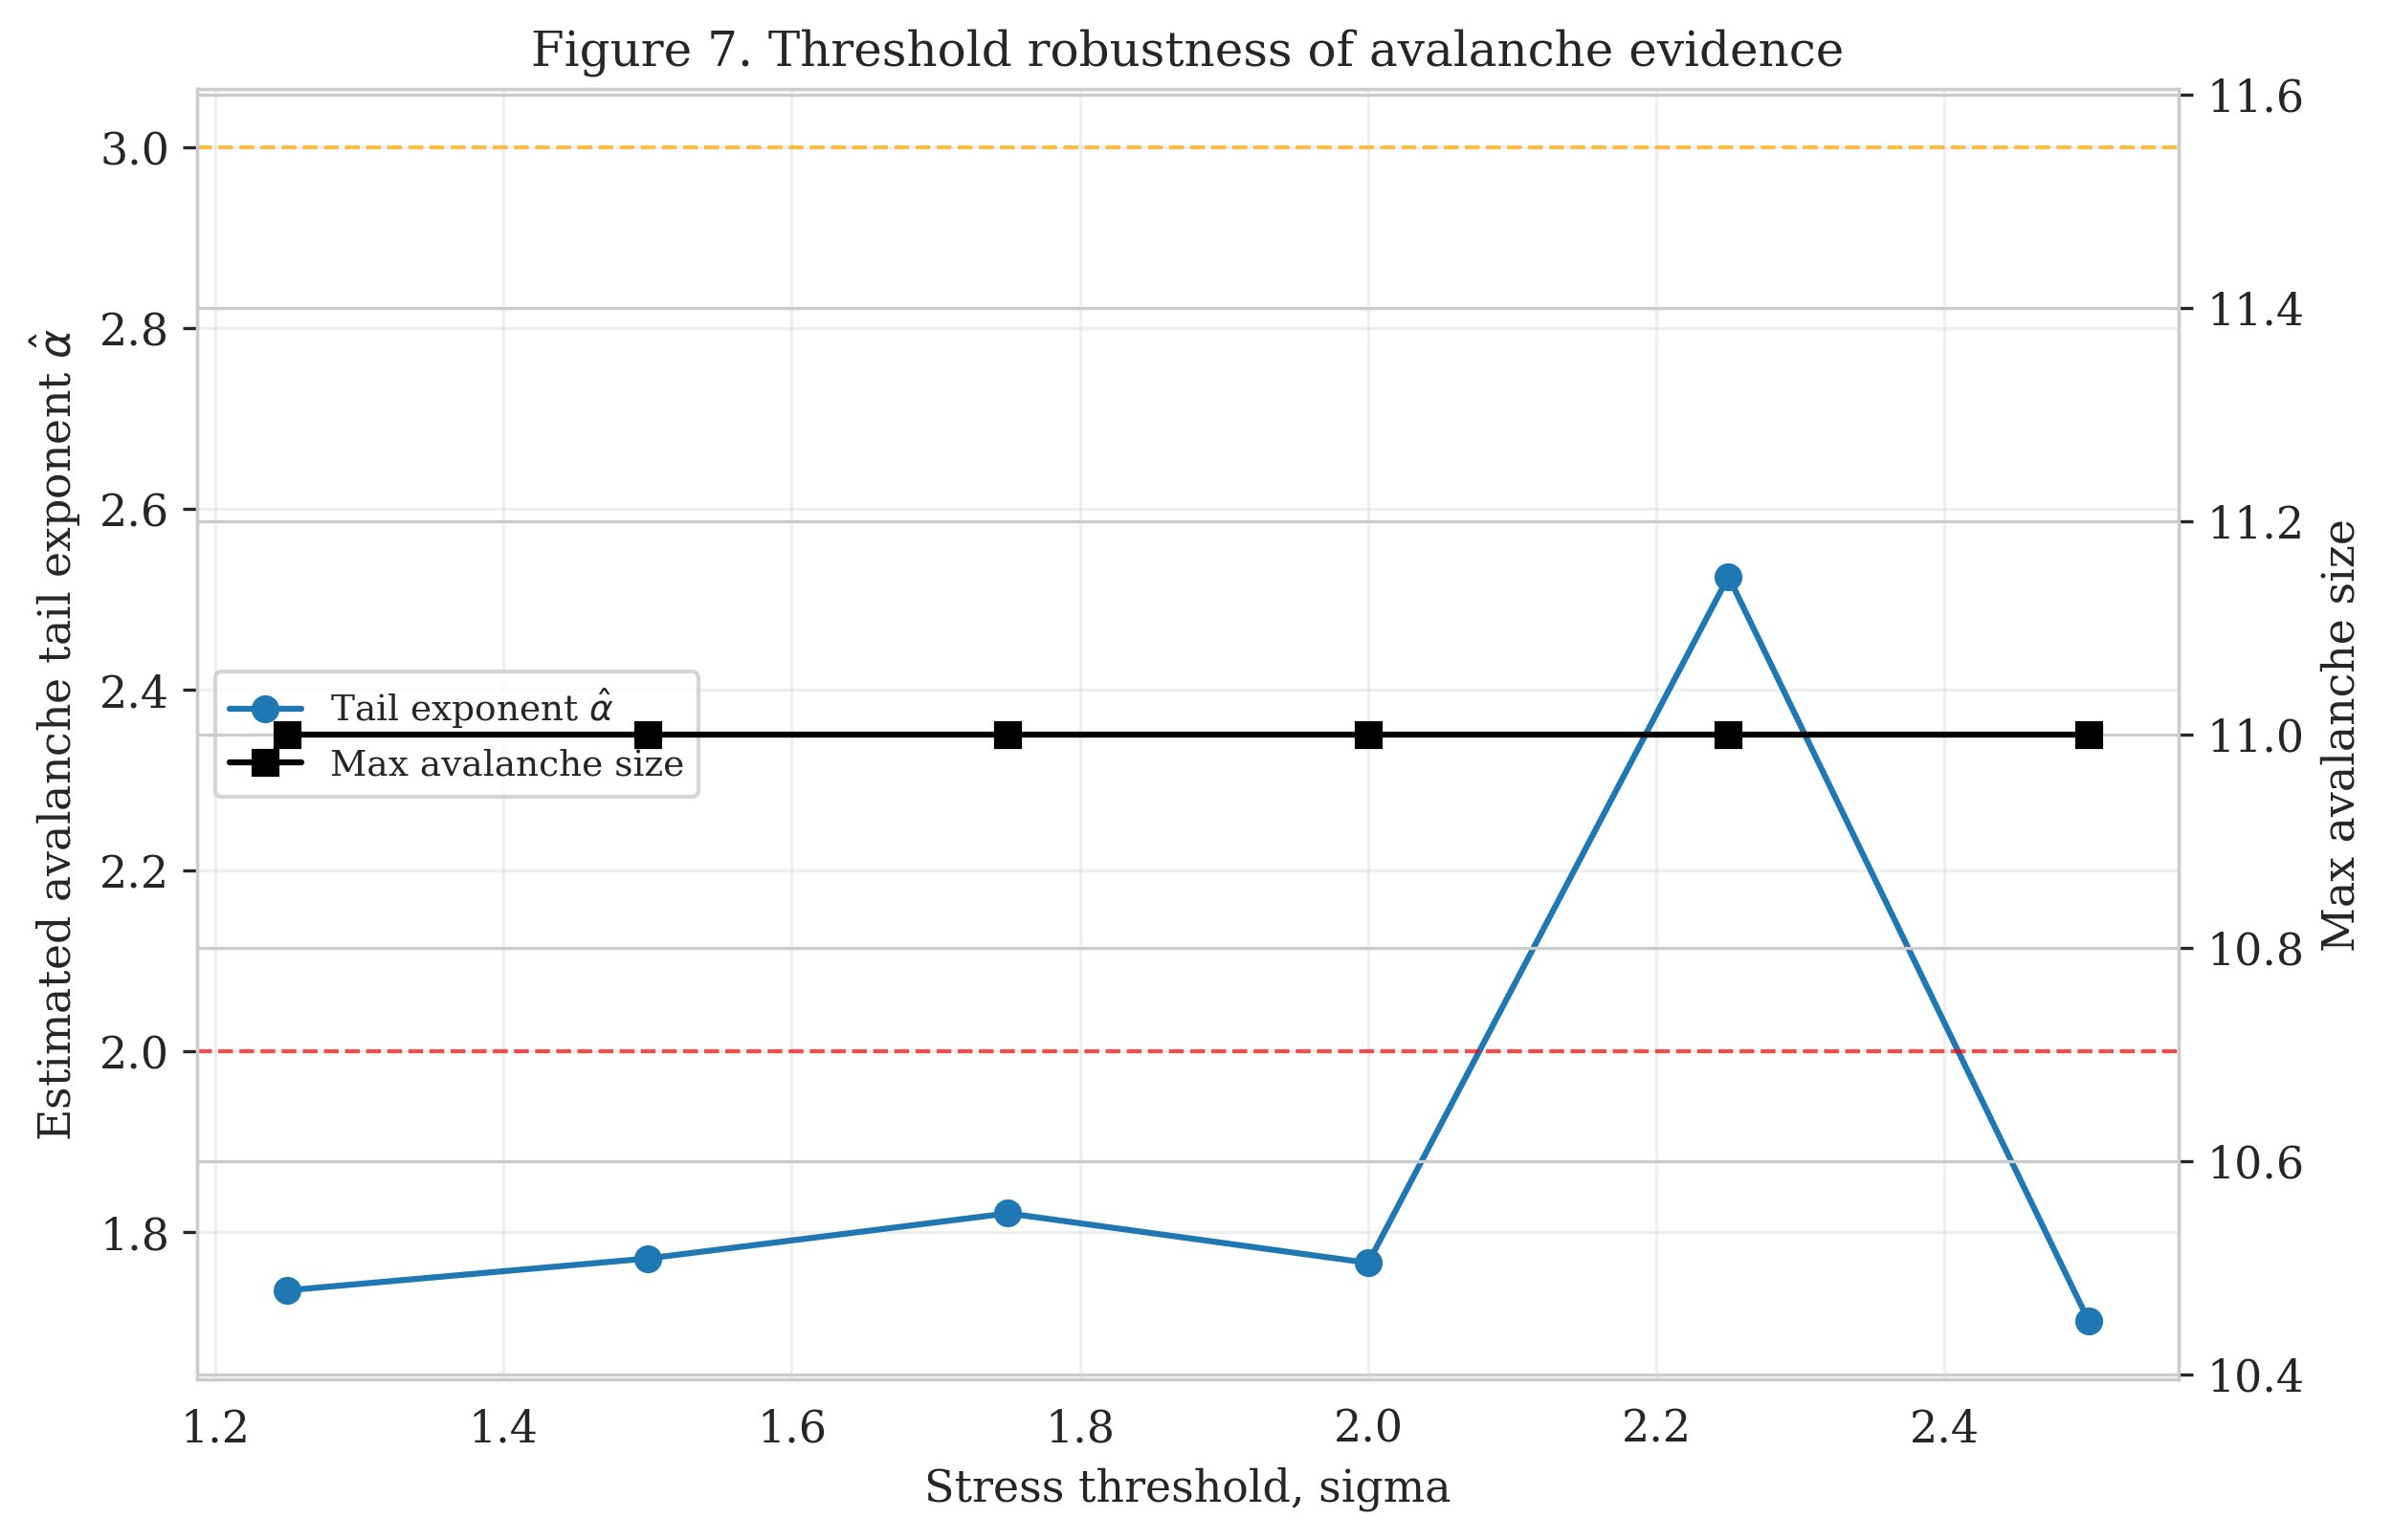
\includegraphics[width=0.9\linewidth]{fig7_threshold_robustness.png}
\caption{Threshold robustness of avalanche evidence. Estimated tail exponent
$\hat{\alpha}$ (left axis, blue) and maximum avalanche size (right axis,
black) as functions of the stress threshold $\sigma\in[1.25, 2.50]$.}
\label{fig:robustness}
\end{figure}

\subsection{Summary of findings}

Table \ref{tab:hypothesis_summary} summarizes the outcome of all six
hypothesis tests. Five hypotheses are confirmed; H5 is partially confirmed
(in the partial-correlation network only). The combined evidence positions
the LATAM sovereign credit system in a heavy-tail boundary regime that is
empirically distinguishable from independence (placebo test), exhibits
country-level heterogeneity organized by financial integration rather than
fiscal stress, and admits operational network-based predictability for
near-future maximum avalanche sizes.

% =============================================================================
\section{Discussion}
\label{sec:discussion}

The empirical evidence positions LATAM sovereign credit in a heavy-tail
boundary regime that is mathematically intermediate between strict power-law
SOC and lognormal heteroscedasticity, but qualitatively distinct from a
Gaussian or sub-critical regime. Three implications follow.

\paragraph{Surveillance.}
The Spectral Fragility Index on partial-correlation networks provides
operational early warning. Both the regime-change discrimination (Table
\ref{tab:network_regime}) and the lead-lag predictability
(Table \ref{tab:network_predictive}) concentrate in this filtering scheme.
Multilateral institutions and central banks could implement monthly SFI
nowcasts at low computational cost. The 24-month rolling window is feasible
with monthly EMBI data and could be cross-validated with weekly or daily
spread series for higher-frequency surveillance. The methodology
complements rather than replaces standard sovereign-spread fundamental
indicators.

\paragraph{Political economy.}
The reformulation of which countries are critical reframes how regional
fragility should be monitored. The standard view treats fiscally stressed
peripheral economies as the prime locus of vulnerability. The data instead
suggest that regional criticality emerges from the well-integrated
mid-credibility sovereigns---Brazil, Mexico, Peru, Colombia, Panama---whose
deeper integration into global EM benchmarks generates more frequent
threshold crossings and thicker network connectivity. ARG and ECU,
counter-intuitively, contribute few avalanche events because their
regime-defining episodes (defaults, FX collapses) saturate the spread in
high absorbed states. Latin American fragility is therefore not the
fragility of its weakest links but of its capital-market integration as a
system.

\paragraph{Theoretical limits.}
The complementary analysis at country level---examining the joint behavior
of country-specific tail exponents and country-level Ollivier--Ricci
curvature---finds no significant association ($r=0.05$, $p=0.45$, see
supplementary material). Aggregate criticality therefore emerges without a
smooth country-by-country curvature--exponent coupling. The relationship
between geometry and criticality is a system property, not a sum of
country properties. This is consistent with the sandpile literature, where
critical behavior is an emergent feature of the global system rather than
a property attributable to individual sites.

\paragraph{Limitations.}
Three caveats apply. First, EMBI data capture only secondary-market spreads;
quantity flows (issuance, foreign holdings) and primary-market funding
costs are not directly observed. Second, the partial-correlation
specification is based on contemporaneous monthly data; richer dynamic
specifications could be implemented at the cost of degrees of freedom.
Third, the MST is informationally limited by its tree structure and may
not reflect the full propagation structure during high-density episodes;
planar maximally filtered graphs \citep{Tumminello2005} could be a
valuable extension.

% =============================================================================
\section{Conclusion}
\label{sec:conclusion}

This paper has tested for self-organized criticality signatures in Latin
American sovereign credit markets using monthly J.P.~Morgan EMBI Global
Diversified spreads for eleven economies over October 2007 to April 2026.
Six formal hypotheses are tested. Five are confirmed and one is partially
confirmed.

The avalanche-size, absolute-spread-change and inter-event-time
distributions all exhibit the heavy-tail boundary regime in the sense of
\citet{StumpfPorter2012}, with power-law fits that cannot be statistically
discriminated from lognormal alternatives but are clearly preferred over
exponentials. Country-level participation in stress events is heterogeneous
and dominated by mid-credibility, financially integrated sovereigns rather
than by high-spread fiscally stressed ones. Cross-country synchronization
is non-trivial: a $B=1{,}000$ reshuffling placebo decisively rejects the
independence null. Partial-correlation network spectral fragility carries
operational predictive content for near-future maximum avalanche size.

The findings complement rather than replace standard fundamental analysis
of sovereign spreads. They suggest a measurement framework that is
particularly suited to regional surveillance, where the joint behavior of
multiple sovereigns matters more than any single country's fiscal
trajectory.

Future work could extend the framework to (i) higher frequency data
(weekly, daily); (ii) other emerging-market regions where EMBI data of
sufficient length exist; (iii) explicit estimation of the structural
mechanism that generates the boundary regime; (iv) integration with
real-economy variables (output, terms of trade, FX) to test causal
direction; and (v) policy-relevant simulations of network-targeted
interventions.

% =============================================================================
\bibliography{references}

\end{document}
